\documentclass[12pt, a4paper, twoside]{article}

\usepackage[dutch]{babel}
\usepackage{hvaTemplate}
% \usepackage[hidelinks]{hyperref}
\usepackage{csquotes}
\usepackage[backend=biber, style=ieee]{biblatex}
\usepackage{pgfplots}
\usepackage{siunitx}
\usepackage{caption}
\usepackage{subcaption}
\usepackage{graphicx}
\usepackage{xspace}
\usepackage{makecell}
\usepackage[perpage]{footmisc}
\usepackage[nameinlink,noabbrev,dutch]{cleveref}
% \usepackage{tikz-among-us}

\sisetup{detect-all}


\pgfplotsset{compat=1.18}

\DeclareMathOperator\erfc{erfc}
\DeclareMathOperator\inverfc{inverfc}
\newcommand\SNR{\mbox{\textit{SNR}} }
\newcommand\SNRout{33}
\newcommand{\mcu}{nRF52810\xspace}
\newcommand\ph{\mathrm{pH}}

% Zorg ervoor dat captions niet lijken op paragrafen
\captionsetup{width=0.85\textwidth}


\DeclareSIUnit{\belmilliwatt}{Bm}
\DeclareSIUnit[scientific-notation = false]{\decibel}{\deci\bel}

\addbibresource{references.bib}

% \setAuthor{\\Tycho Jöbsis (500845792)\\ Jochem Leijenhorst (500855372)\\ Illya Ustenko (500845492)}
\setAuthor{
    \\Groep 7
    \begin{table}[h!]
        \centering
        \begin{tabular}{ll}
            Jochem Leijenhorst  & (500855372)\\
            Tycho Jöbsis        & (500845792)\\
            Illya Ustenko       & (500845492)
        \end{tabular}
    \end{table}
}
\extraInfo{Sensor modules}
\setTitle{Ontwerptraject pH sensor}

\graphicspath{ {img/} }

\numberwithin{equation}{section}

\DeclareSIUnit{\pH}{pH}

\makeatletter
\providecommand\add@text{}
\newcommand\tagaddtext[1]{%
\gdef\add@text{#1\gdef\add@text{}}}%
\renewcommand\tagform@[1]{%
  \maketag@@@{\llap{\add@text\quad}(\ignorespaces#1\unskip\@@italiccorr)}%
}
\makeatother

\begin{document}
    \makeTitlepage
    % \begin{tikzpicture}
    %     \amongUsI{yellow}{cyan}
    %     \hspace{10cm}
    %     \amongUsI{red}{cyan}
    % \end{tikzpicture}

    In dit ontwerpverslag wordt het ontwerptraject van een energiezuinige, pH metende sensormodule besproken. Deze sensormodule maakt gebruik van een ISFET pH sensor om de pH waarde van een oplossing te kunnen meten.
De gemeten pH waarde wordt draadloos verstuurd naar een basisstation. De sensormodule beschikt ook over een Energy Harvesting systeem, die bedoelt is om de levensduur van de module te verlengen.
Het is uiteindelijk deels gelukt om zo'n sensormodule te realiseren; De ISFET uitleesschakeling gedraagt zich op dit moment nog niet zoals verwacht. De module verbruikt in totaal gemiddeld \qty{6.84}{\milli\watt}.


In this design report, the design of an energy-efficient pH-sensing sensor module is discussed. The sensor module utilizes an ISFET pH sensor to measure the pH level of a solution.
The measured pH value is transmitted wirelessly to a base-station. The module is also capable of harvesting energy, which is used to prolong the battery life of the module.
The realization of the sensor module was partially successful; The ISFET readout circuit currently does not function as expected. The total average power consumption of the module is \qty{6.84}{\milli\watt}.

    \onecolumn
    \tableofcontents


    \newpage

    \section{Inleiding}

Voor het doen van onderzoek naar productiemethoden van drinkwater, is het belangrijk om tijdens verscheidene productie stappen de pH-waarde van het water te kunnen meten. Om dat mogelijk te maken zal er in dit project gewerkt worden aan een eerste prototype van een pH-sensormodule. Deze sensormodule zal rondom een ion gevoelige veld effect transistor (ISFET) worden ontwikkeld. De reden dat er geen gebruik gemaakt wordt van een glazen electrode pH-sensoren is omdat deze duurder zijn om te produceren \cite{duroux1991ionpHISFETltspHmonitoring}.

In het onderzoek waar deze sensormodule voor wordt ontwikkeld, zullen er meerdere van deze modules voor langere tijd data verzamelen. Om het makkelijk te maken om de pH meetdata te verzamelen heeft de sensormodule een draadloze verbinding nodig. Via deze draadloze verbinding is het dan mogelijk om de meetdata naar een basisstation te sturen. Dit basisstation is al ontwikkeld.

Verder zal er gekeken worden naar methodes van energie harvesting om de levensduur van de sensormodule te verlengen.

    \newpage

    \section{Theoretisch kader}
Voordat er ontworpen kan worden zal er eerst onderzoek gedaan moeten worden naar de werking van een ISFET. Dit is nodig om te weten hoe de pH waarde van de oplossing waar de ISFET zich in bevindt uit te lezen valt.
Hiernaast zal er, omdat de module zichzelf ook moet kunnen opladen, ook onderzoek gedaan moeten worden naar energy harvesting.
Dit hoofdstuk zal ingaan op de bevindingen van het onderzoeken van beide onderwerpen.

\subsection{De werking van de ISFET}\label{sec:werkingISFET}
Een ISFET (Ion-Sensitive Field-Effect Transistor) is een FET die gevoelig is voor ionen. Hierdoor is het mogelijk om er pH-waardes mee te meten\cite{modeling}. Een ISFET is in principe een MOSFET zonder gate. De ISFET gedraagt zich in de eerste instantie ook als transistor. Er wordt een referentie-elektrode aan de te meten oplossing toegevoegd om de pH-waarde te kunnen meten. Deze referentie-elektrode kan gebruikt worden als de gate van de MOSFET\cite{van1987isfet}. De drempelspanning van de transistor is echter een functie van de pH-waarde van de gemeten oplossing. Een hogere pH-waarde geeft een lagere drempelspanning\cite{isfet}.

De ISFET is temperatuursafhankelijk\cite{isfet}. Volgens de datasheet is de temperatuursafhankelijkheid gemiddeld $\qty{-0.2}{\milli\volt\per\kelvin}$\cite{Microsens-MSFET}. Om hiervoor te compenseren moet tijdens het meten ook de temperatuur gemeten worden. Daarbij zal bij het kalibreren de kalibratietemperatuur opgeslagen moeten worden. Wanneer vervolgens gemeten wordt, zal de gemeten spanning door middel van het temperatuurverschil gecompenseerd moeten worden. Deze compensatie kan gedaan worden door middel van \cref{eq:tempComp}.

\begin{equation}\label{eq:tempComp}
    U_r = U_m + C_T(T_{meting} - T_{kalibratie})
    \tagaddtext{[\si{\volt}]}
\end{equation}
Hierbij is $U_r$ de op temperatuur gecompenseerde ingangsspanning en $U_m$ de gemeten spanning.

De richtingscoëfficiënt tussen de pH-waarde en de drempelspanning is constant, en varieert alleen van ISFET tot ISFET. Door deze als constant te nemen kan de pH-waarde berekend worden met een enkel kalibratiepunt.

\begin{equation}\label{eq:calcPH}
    \ph = C_{ph}(U_r - U_k) + \ph_k
    \tagaddtext{[pH]}
\end{equation}
Hierbij is $a$ de richtingscoëfficiënt van de ISFET in pH/V, $U_r$ de op temperatuur gecompenseerde ingangsspanning, $\ph_k$ de pH waarde tijdens de kalibratie en $U_k$ de gemeten kalibratiespanning.

\subsection{Empirisch onderzoek}
% \subsection{Gebruikersonderzoek}
% \subsection{Methodes}


\subsection{Energy Harvesting}
In veel toepassingen is het nuttig dat een sensormodule weinig onderhoud nodig heeft. Daarbij is het batterijleven van de sensormodule een van de belangrijkste aspecten. Energy harvesting is een manier om de levensuur van apparaten aanzienlijk te kunnen vergroten. Hierbij wordt energie uit de omgeving omgezet naar bruikbare elektrische energie. Er zijn meerdere methodes om energie te verkrijgen uit de omgeving. Voorbeelden van mogelijke energiebronnen zijn \cite{energyHarvesting}:
\begin{itemize}
    \item Kinetische energie
    \begin{itemize}
        \item Wind
        \item Water
        \item Vibratie
    \end{itemize}
    \item Elektromagnetische energie
    \begin{itemize}
        \item Zonne energie
        \item Radio-frequentie
    \end{itemize}
    \item Thermische energie
    \item Atomische energie
    \begin{itemize}
        \item Radioactief verval
    \end{itemize}
\end{itemize} 

Deze energiebronnen wekken energie op die door de sensor module accu kan worden opgeslagen. Om er een methode te kiezen is het belangrijk om te kijken naar de omgeving waar het module gebruikt gaat worden. Volgens de opdrachtgevers (groep onderzoekers) kan de sensor module binnen worden ingezet. Hierdoor valt een deel van de mogelijke energiebronnen al af: wind en zonne energie. Daarbij is wordt het sensor module gebruikt in een industriële omgeving. Binnen industriële omgevingen worden veel pompen en andere apparaten gebruikt die vibratie veroorzaken. Hierdoor zou je vibratie goed kunnen gebruiken om energie uit te halen. Voor het energie 

% \subsubsection{Voor en nadelen van energiebronnen}

% \begin{table}[!htbp]
%     \centering
%     \begin{tabular}{ | l | c | c | c | }
%         \hline
%         Energiebron & Voordelen & Nadelen \\
%         \hline
%         Wind &   \\
%         Water   \\
%         Vibratie   \\
%         Elektromagnetisme     \\
%         Zonne     \\
%         Radio-frequentie   \\
%         Thermische     \\
%         Atomische     \\
%         Radioactief verval   \\
%         \hline
%     \end{tabular}
%     \caption{Voor en nadelen energiebronnen}
%     \label{tab:fuckingKanker}
% \end{table}




    \newpage

    \section{Specificaties}
De pH sensor moet met grote nauwkeurigheid de pH waarde van een stof continu kunnen meten. 
De enige beschikbare pH sensor die dit kan doen is een ISFET.
Hierdoor zijn de specificaties deels gebaseerd op de specificaties van een ISFET pH sensor.

De sensormodule heeft een eigen accu, en moet deze op kunnen laden zonder oplaadkabel.

\begin{table}[ht]
    \centering
    \begin{tabular}{|l|c c|l|c|}
        \hline
        Beschrijving                 & Min & Max  & Eenheid   & Bron \\
        \hline 
        Gemiddeld gebruikte vermogen &     & 10   & mW        & Opdrachtgever \\
        Afwijking                    &     & 0.05 & pH        & \cite{isfet} \\ 
        % Temperatuur                  &     &      & $^\circ$C & ???           \\
        Bereik                       & 2   & 10   & pH        & \cite{isfet} \\
        Metingssnelheid              & 1   &      & S/s       & \cite{isfet} \\
        Bandbreedte                  & 10  &      & Hz        & Opdrachtgever\\
        $\mathrm{SNR}_{uit}$         & 36  & 36   & dBm       &  \\
        \hline
    \end{tabular}
    \caption{Systeemspecificaties.}
    \label{tab:systemSpecs}
\end{table}


% BER 0.01%


% \begin{table}[ht]
%     \centering
%     \begin{tabular}{|l|r|}
%         \hline
%         BER             & 0.01\%  \\
%         Energie per bit & J/b \\
%         SNR             & \% \\
%         Gevoeligheid Ontvanger & \% \\
%         Zendvermogen    & dBm \\
%         Ez              & \\ 
%         Data rate       & b/s\\
%         \hline
%     \end{tabular}
%     \caption{Specificaties draadloze verbinding.}
%     \label{tab:wirelessSpec}
% \end{table}


    \newpage

    \section{Ontwerp}\label{sec:ontwerp}
Het systeem bestaat uit 2 hoofdonderdelen: de sensormodule en een basisstation. De sensormodule meet de pH waarde van een oplossing, en verzend deze naar het basisstation. Het basisstation ontvangt de informatie en slaat deze informatie op.
In \cref{fig:functional} is dit te zien in een systeemdiagram.

\begin{figure}[ht]
    \centering
    \includegraphics{toplevelDiagram}
    \caption[short]{Een diagram van het volledige systeem.}
    \label{fig:functional}
\end{figure}

Het sensormodule blok kan wederom opgedeeld worden in aparte blokken. Dit is te zien in \cref{fig:moduleDiagram}.

\begin{figure}[ht]
    \centering
    \includegraphics[width=0.75\textwidth]{moduleDiagram}
    \caption{Een systeemdiagram van de sensormodule.} 
    \label{fig:moduleDiagram}
\end{figure}

\subsection{Functionele decompositie}
De sensormodule kan opgedeeld worden in 2 aparte systemen: de voeding, die verder wordt besproken in \cref{sec:voeding}, en de signaalverwerking.

De signaalverwerking bestaat zelf ook weer uit 2 onderdelen: het analoge gedeelte en het digitale gedeelte. In \cref{fig:analogeBewerkingsFunctie} is een decompositie te zien van de signaalbewerkingsfuncties die toegepast worden in het analoge gedeelte. In de komende paragrafen wordt elk van deze blokken apart besproken.

\begin{figure}[ht]
    \centering
    \includegraphics[width=0.95\textwidth]{analogeBewerkingsFunctie}
    \caption{Het analoge gedeelte van de signaalbewerking.} 
    \label{fig:analogeBewerkingsFunctie}
\end{figure}


Het digitale gedeelte bestaat uit een aantal berekeningen. Deze berekeningen zijn nodig om de gemeten spanning om te rekenen naar een pH waarde. Hiervoor zijn een aantal kalibratiewaardes nodig, zoals besproken in \cref{sec:werkingISFET}. Het digitale gedeelte heeft als ingang een temperatuursafhankelijke spanning $U_T$ en een pH-afhankelijke spanning $U_{pH}$. Dit is te zien in \cref{fig:digitaleBewerkingsFunctie}. Beide van deze spanningen zijn de ruwe ADC waardes die gemeten worden, en hebben dus de hoogst mogelijke resolutie, namelijk de resolutie van de ADC. Voor beide van deze waardes zal de eenheid `bit' gebruikt worden.

Om op de uiteindelijk pH waarde te komen, wordt van de pH-afhankelijke spanning de pH-afhankelijke kalibratiespanning afgetrokken. Vervolgens wordt hier $\frac{pH_{kal}}{C_{pH}}$ bij opgeteld. Op deze manier kan er zo lang mogelijk met integers gewerkt worden die dezelfde resolutie hebben als de ingangs-ADC waarde. Het resultaat wordt vervolgens vermenigvuldigd met $C_{pH}$. Dit is de gevoeligheid van de sensor, in pH/bit.

Om de temperatuursafwijking te berekenen, wordt eerst van de temperatuursafhankelijke spanning $U_T$ de temperatuursafhankelijke kalibratiespanning $U_{T,kal}$ afgetrokken. Vervolgens wordt dit vermenigvuldigt met constante $C_T$. $C_T$ is de temperatuursafhankelijkheid van de pH-sensor, in pH/bit. Deze waarde kan afgeleid worden met de temperatuursafhankelijkheid van de pH-sensor die in de datasheet gegeven wordt in mV/K \cite{isfet}.

\begin{figure}[ht]
    \centering
    \includegraphics[width=0.95\textwidth]{digitaleBewerkingsFunctie}
    \caption{Het digitale gedeelte van de signaalbewerking.} 
    \label{fig:digitaleBewerkingsFunctie}
\end{figure}


\section{De drempelspanning van de ISFET uitlezen}

% TODO: Bronnen
Om de pH waarde van de ISFET uit te lezen moet de drempelspanning gemeten worden. Deze is namelijk linear afhankelijk van de pH waarde.
Om de drempelspanning te meten kan een regelsysteem gebruikt worden. Door de gate-source spanning te variëren kan de spanning over en de stroom door de drain en de source van de ISFET gelijk gehouden worden.

Er zijn meerdere mogelijke implementaties van een dergelijk regelsysteem. In \autoref{fig:measureCircuits} staan er drie.
Elk van deze schakelingen gebruikt een nullor om de drain-source spanning van de ISFET gelijk te houden. Ook gebruikt elk van deze schakelingen een referentiespanning. De implementatie van deze referentiespanning wordt verder besproken in \autoref{sec:referenceVoltage}.

De drain-source spanning $U_{ds}$ en drain-source stroom $I_{ds}$ zijn van te voren gedefinieerd. Deze zijn ook te vinden in de datasheet van de ISFET\cite{isfet}. Uit deze twee waardes kunnen de referentiespanningen en weerstandswaardes van de schakelingen gevonden worden.
Voor de schakeling in \autoref{fig:measureCurrent} is de spanningsreferentie te vinden door middel van \autoref{eq:URefSource}.
\begin{equation}\label{eq:URefSource}
    U_{ref,s} = U_{dd} - U_{ds}
\end{equation}
Voor \autoref{fig:measureResistor} is de referentiespanning gelijk aan de drain-source spanning.
\begin{equation}\label{eq:URefDrain}
    U_{ref,d} = U_{ds}
\end{equation}
Voor de waarde van de weerstand in \autoref{fig:measureResistor} kan \autoref{eq:measureResistorVal} gebruikt worden.
\begin{equation}\label{eq:measureResistorVal}
    R = \frac{U_{dd} - U_{ds}}{I_{ds}}
\end{equation}


\begin{figure}[ht]
    \centering
    \begin{subfigure}[b]{0.45\textwidth}
        \centering
        \def\svgwidth{\textwidth}
        \input{img/ISFETCircuitBest.pdf_tex}
        \caption{Met een weerstand aan de drain.}
        \label{fig:measureResistor}
    \end{subfigure}
    \hfill
    \begin{subfigure}[b]{0.45\textwidth}
        \centering
        \def\svgwidth{\textwidth}
        \input{img/ISFETCircuit.pdf_tex}
        \caption{Met een stroombron.}
        \label{fig:measureCurrent}
    \end{subfigure}
    \caption{De uitleesschakelingen voor de ISFET.}
    \label{fig:measureCircuits}
\end{figure}

Beide schakelingen heeft voor- en nadelen.
Bij de schakeling in \autoref{fig:measureResistor} zit de source van de ISFET direct verbonden met de aarde. Dit heeft als voordeel dat de uitgang van de nullor gelijk is aan de gate-source spanning. Hierdoor hoeft de nullor lagere spanningen te genereren om de gate-source spanning van de mosfet naar de goede waarde te krijgen. De spanning die de nullor moet genereren in het geval van een drain weerstand is te vinden door middel van \autoref{eq:nullorVoltageDrain}. In het geval van een stroombron aan de source is dat \autoref{eq:nullorVoltageSource}.

\begin{equation}\label{eq:nullorVoltageDrain}
    U_{nullor,d} = U_{gs}
    \tagaddtext{[\si{\volt}]}
\end{equation}
\begin{equation}\label{eq:nullorVoltageSource}
    U_{nullor,s} = U_{gs} + U_{ref,s}
    \tagaddtext{[\si{\volt}]}
\end{equation}

De schakeling met een stroombron aan de source heeft de mogelijkheid om betere ruiseigenschappen te hebben. De stroombron kan ook een hogere impedantie hebben dan de weerstand, wat goed is volgens mij. 

\newcommand\ph{\mathrm{pH}}

De meetschakeling heeft een aantal ruisbronnen. De nullor heeft een ingangsstroom- en spanninsruisbron. Daarnaast genereert de weerstand ook thermische ruis. Deze ruisbronnen zijn te zien in \autoref{fig:measureNoise}.
\begin{figure}[ht]
    \centering
    \def\svgwidth{0.6\textwidth}
    \input{img/ISFETCircuitBestNoise.pdf_tex}
    \caption{De ruisbronnen van de meetschakeling.}
    \label{fig:measureNoise}
\end{figure}

De overdracht van deze schakeling is gelijk aan de uitgangsspanning gedeeld door de ingangsspanning van de nullor. Door de werking van de schakeling blijft de ingansspanning altijd gelijk en is de uitgangsspanning lineair afhankelijk van de pH waarde. Hierdoor is de overdracht $H(\ph)$ een functie van de gemeten pH waarde.
Omdat $U_{ds}$ en $I_{ds}$ van de ISFET niet veranderen, kan de impedantie ervan gezien worden als weerstand, met een waarde van $\frac{U_{ds}}{I_{ds}}$. Hierdoor wordt er een nieuwe ruisbron $i_{n,ds}$ toegevoegd. Met deze weerstand kunnen de bronnen $i_{n,ref}$, $i_{n,R}$ en $i_{n,ds}$ worden getransformeerd naar een spanningsbron $u{n,in}$ aan de ingang van de nullor.
Vervolgens kan deze, samen met de spanningsruisbronnen $u_{n,ref}$ en $u_{n,n}$ naar de uitgang getransformeerd worden. Dit komt uit op een spanningsruisbron aan de uitgang, zoals te zien in \autoref{fig:measureNoiseMoved}. De spectrale spanningsruisdichtheid hiervan is te berekenen door middel van \autoref{eq:measureNoiseOut}.

\begin{equation}\label{eq:measureNoiseOut}
    Su_{n,out} = \left(Su_{n,ref} + Su_{n,n} + Si_{n,in}\left(Z_{fet} // R\right)^2\right) \cdot H^2(\ph)
    \tagaddtext{[\si{\volt\squared\per\hertz}]}
\end{equation}
\begin{equation}
    Si_{n,in} = Si_{n,n} + Si_{n,R} + Si_{n,ds}
    \tagaddtext{[\si{\ampere\squared\per\hertz}]}
    \label{eq:measureNoiseCurrentIn}
\end{equation}


De waardes van deze ruisbronnen zijn te vinden in \autoref{tab:measureNoiseValues}.

\begin{table}[ht]
    \centering
    \begin{tabular}{c|l}
        Ruisbron & Waarde \\
        \hline 
        $Su_{n,ref}$ & Zie \autoref{sec:referenceVoltage} \\
        $Su_{n,n}$   & Implementatie nullor \\
        $Si_{n,n}$   & Implementatie nullor \\
        $Si_{n,R}$   & $\frac{4kT}{R}$ \\
        $Si_{n,ds}$  & $4kT\frac{I_{ds}}{U_{ds}}$ \\
    \end{tabular}
    \caption{Waar de waardes van de ruisbronnen vandaan gehaald kunnen worden.}
    \label{tab:measureNoiseValues}
\end{table}

\begin{figure}[ht]
    \centering
    \def\svgwidth{0.6\textwidth}
    \input{img/ISFETCircuitBestNoiseMoved.pdf_tex}
    \caption{De meetschakeling met verschoven ruisbronnen.}
    \label{fig:measureNoiseMoved}
\end{figure}
\subsection{Spanningsreferentie}\label{sec:referenceVoltage}

De ISFET uitleesschakeling heeft een spanningsreferentie nodig om te werken. Deze spanningsreferentie kan op meerdere manieren gegenereerd worden.
% TODO: Vertel misschien over andere methoden.
Uiteindelijk is er een spanningsdeler gekozen om de spanningsreferentie mee te implementeren. De schakeling van deze spanningsdeler is te zien in \autoref{fig:divider}.
De condensator wordt gebruikt om ruis te verminderen op hogere frequenties, en dient ook als filter voor hoogfrequente fouten in de voedingsspanning.

\begin{figure}[ht]
    \centering
    \def\svgwidth{0.5\textwidth}
    \subsection{Spanningsreferentie}\label{sec:referenceVoltage}

De ISFET uitleesschakeling heeft een spanningsreferentie nodig om te werken. Deze spanningsreferentie kan op meerdere manieren gegenereerd worden.
% TODO: Vertel misschien over andere methoden.
Uiteindelijk is er een spanningsdeler gekozen om de spanningsreferentie mee te implementeren. De schakeling van deze spanningsdeler is te zien in \autoref{fig:divider}.
De condensator wordt gebruikt om ruis te verminderen op hogere frequenties, en dient ook als filter voor hoogfrequente fouten in de voedingsspanning.

\begin{figure}[ht]
    \centering
    \def\svgwidth{0.5\textwidth}
    \input{img/divider.pdf_tex}
    \caption{De schakeling van de spanningsdeler die dient als spanningsreferentie.}
    \label{fig:divider}
\end{figure}

\noindent
De overdracht van deze spanningsdeler is te vinden in \autoref{eq:dividerTransfer}.
\begin{equation}\label{eq:dividerTransfer}
    H(s) = \frac{U_{ref}(s)}{U_{dd}(s)} = \frac{R_2}{R_1 + R_2 + R_2Cs}
\end{equation}

\noindent
Het vermogen dat de spanningsdeler dissipeert, kan met \autoref{eq:dividerPower} berekend worden.
\begin{equation}\label{eq:dividerPower}
    P(s) = U_{dd}(s)^2\frac{1+R_2Cs}{R_1 + R_2 + R_1R_2Cs}
\end{equation}
Met een constante DC ingangsspanning kan dit vereenvoudigd worden naar \autoref{eq:dividerPowerSimple}.
\begin{equation}\label{eq:dividerPowerSimple}
    P = \frac{U_{dd}^2}{R_1 + R_2}
\end{equation}

\noindent
Om de ruis van deze schakeling te berekenen moet een aantal stappen genomen worden. Aangezien de ingangsbron $U_{dd}$ een spanningsbron is, kan deze als kortsluiting genomen worden. Op deze manier kunnen de twee weerstanden parallel genomen worden, en verandert de schakeling in een simpel RC filter. In \autoref{fig:dividerNoise} is deze omgebouwde schakeling te zien.

\begin{figure}[ht]
    \centering
    \def\svgwidth{0.35\textwidth}
    \input{img/dividerNoise.pdf_tex}
    \caption{De omgebouwde schakeling om ruis mee te berekenen.}
    \label{fig:dividerNoise}
\end{figure}

\noindent
Voor de spectrale spanningsruisdichtheid aan de uitgang $U_{ref}$ kan \autoref{eq:dividerNoiseLaplace} worden opgesteld.
\begin{equation}\label{eq:dividerNoiseLaplace}
    S_{n,u_{ref}} = 4kTR_e\left(\frac{1}{1 + R_eCs}\right)^2
\end{equation}
Wanneer de absolute waarde van de ruis wordt genomen, kan deze over de bandbreedte geïntegreerd worden. Dit resulteert in \autoref{eq:dividerNoiseInt}.
\begin{equation}\label{eq:dividerNoiseInt}
    u_{n,ref}^2 = \int_{\omega_l}^{\omega_h} 4kTR_e\left(\frac{1}{\sqrt{1 + (R_eC\omega)^2}}\right)^2 d\omega
\end{equation}
Het integraal van deze formule komt uit op \autoref{eq:dividerNoiseIntegrated}.
\begin{equation}\label{eq:dividerNoiseIntegrated}
    u_{n,ref}^2 = \frac{4kT}{C}\left[\arctan(R_eC\omega_h) - \arctan(R_eC\omega_l)\right]
\end{equation}

Zolang de spanning stabiel is hoeft de referentie geen exact gedefinieerde spanning te hebben. Dit is omdat de ADC die de waarde van de sensor gaat uitlezen deze referentiespanning ook als referentie zal gebruiken. De waarde moet echter ergens rond de 1.1V zitten, om de stroombron te laten werken.
In \autoref{sec:currentSource} is hier meer over te lezen.
Aangezien de ingangsspanning 1.8V is, zal de DC overdracht $1.1 / 1.8 = \frac{11}{18}$ zijn. Hieruit komt de weerstandsverhouding in \autoref{eq:dividerResistors}.
\begin{equation}\label{eq:dividerResistors}
    \frac{R_1}{R_2} = \frac{7}{11}
\end{equation}
Een hogere $R_1$ zorgt voor een lager vermogensverbruik, maar ook een hogere ruis. Dit is te zien in \autoref{fig:dividerPlots}.

\begin{figure}
    \centering
    \begin{subfigure}[b]{0.45\textwidth}
        \centering
        \input{plots/dividerNoise}
        \caption{Spanningsruis}
        \label{fig:dividerNoisePlot}
    \end{subfigure}
    \hfill
    \begin{subfigure}[b]{0.45\textwidth}
        \centering
        \input{plots/dividerPower}
        \caption{Vermogensverbruik}
        \label{fig:dividerPower}
    \end{subfigure}
    \caption{De ruis en het vermogensverbruik van de spanningsdeler, ten opzichte van de gekozen weerstandswaarde $R_1$.}
    \label{fig:dividerPlots}
\end{figure}
Op $R_1 = 1\si{\mega\ohm}$ en $C = 10\si{\micro\farad}$ is de spanningsruis $u_{n,ref} = 51\si{\nano\volt}$ en het vermogensverbruik $P = 1.3\si{\micro\watt}$. De andere weerstandswaarde is dan $R_2 \approx 1.6 \si{\mega\ohm}$. Deze waardes vallen binnen de specificaties.

[WELKE SPECS??]
    \caption{De schakeling van de spanningsdeler die dient als spanningsreferentie.}
    \label{fig:divider}
\end{figure}

\noindent
De overdracht van deze spanningsdeler is te vinden in \autoref{eq:dividerTransfer}.
\begin{equation}\label{eq:dividerTransfer}
    H(s) = \frac{U_{ref}(s)}{U_{dd}(s)} = \frac{R_2}{R_1 + R_2 + R_2Cs}
\end{equation}

\noindent
Het vermogen dat de spanningsdeler dissipeert, kan met \autoref{eq:dividerPower} berekend worden.
\begin{equation}\label{eq:dividerPower}
    P(s) = U_{dd}(s)^2\frac{1+R_2Cs}{R_1 + R_2 + R_1R_2Cs}
\end{equation}
Met een constante DC ingangsspanning kan dit vereenvoudigd worden naar \autoref{eq:dividerPowerSimple}.
\begin{equation}\label{eq:dividerPowerSimple}
    P = \frac{U_{dd}^2}{R_1 + R_2}
\end{equation}

\noindent
Om de ruis van deze schakeling te berekenen moet een aantal stappen genomen worden. Aangezien de ingangsbron $U_{dd}$ een spanningsbron is, kan deze als kortsluiting genomen worden. Op deze manier kunnen de twee weerstanden parallel genomen worden, en verandert de schakeling in een simpel RC filter. In \autoref{fig:dividerNoise} is deze omgebouwde schakeling te zien.

\begin{figure}[ht]
    \centering
    \def\svgwidth{0.35\textwidth}
    \begin{tikzpicture}
    \pgfplotsset{width=\textwidth}
    \newcommand\BOLZ{1.380649e-23}
    \newcommand\TEMP{300}
    \newcommand\OMEGAC{15*2*pi}
    \newcommand\RESRAT{(7/11)}
    \newcommand\REQU{(1/(1/x + \RESRAT/x))}
    \newcommand\CAP{0.000001}

    \pgfplotsset{set layers}
    \begin{axis}[
        xmode=log,
        ymode=log,
        xlabel={$R_1 [\si{\ohm}]$},
        ylabel={$u_{n,out} [\si{\volt}]$},
        xmin=1e3, xmax=1e7,
        grid=major
    ]

    \addplot [
        red,
        domain=1e3:1e7,
        samples=201
    ]
    {sqrt((4 * \BOLZ * \TEMP / \CAP) * rad(atan(\REQU * \CAP * \OMEGAC)))};
    \end{axis}
\end{tikzpicture}
    \caption{De omgebouwde schakeling om ruis mee te berekenen.}
    \label{fig:dividerNoise}
\end{figure}

\noindent
Voor de spectrale spanningsruisdichtheid aan de uitgang $U_{ref}$ kan \autoref{eq:dividerNoiseLaplace} worden opgesteld.
\begin{equation}\label{eq:dividerNoiseLaplace}
    S_{n,u_{ref}} = 4kTR_e\left(\frac{1}{1 + R_eCs}\right)^2
\end{equation}
Wanneer de absolute waarde van de ruis wordt genomen, kan deze over de bandbreedte geïntegreerd worden. Dit resulteert in \autoref{eq:dividerNoiseInt}.
\begin{equation}\label{eq:dividerNoiseInt}
    u_{n,ref}^2 = \int_{\omega_l}^{\omega_h} 4kTR_e\left(\frac{1}{\sqrt{1 + (R_eC\omega)^2}}\right)^2 d\omega
\end{equation}
Het integraal van deze formule komt uit op \autoref{eq:dividerNoiseIntegrated}.
\begin{equation}\label{eq:dividerNoiseIntegrated}
    u_{n,ref}^2 = \frac{4kT}{C}\left[\arctan(R_eC\omega_h) - \arctan(R_eC\omega_l)\right]
\end{equation}

Zolang de spanning stabiel is hoeft de referentie geen exact gedefinieerde spanning te hebben. Dit is omdat de ADC die de waarde van de sensor gaat uitlezen deze referentiespanning ook als referentie zal gebruiken. De waarde moet echter ergens rond de 1.1V zitten, om de stroombron te laten werken.
In \autoref{sec:currentSource} is hier meer over te lezen.
Aangezien de ingangsspanning 1.8V is, zal de DC overdracht $1.1 / 1.8 = \frac{11}{18}$ zijn. Hieruit komt de weerstandsverhouding in \autoref{eq:dividerResistors}.
\begin{equation}\label{eq:dividerResistors}
    \frac{R_1}{R_2} = \frac{7}{11}
\end{equation}
Een hogere $R_1$ zorgt voor een lager vermogensverbruik, maar ook een hogere ruis. Dit is te zien in \autoref{fig:dividerPlots}.

\begin{figure}
    \centering
    \begin{subfigure}[b]{0.45\textwidth}
        \centering
        \begin{tikzpicture}
    \pgfplotsset{width=\textwidth}
    \newcommand\BOLZ{1.380649e-23}
    \newcommand\TEMP{300}
    \newcommand\OMEGAC{15*2*pi}
    \newcommand\RESRAT{(7/11)}
    \newcommand\REQU{(1/(1/x + \RESRAT/x))}
    \newcommand\CAP{0.000001}

    \pgfplotsset{set layers}
    \begin{axis}[
        xmode=log,
        ymode=log,
        xlabel={$R_1 [\si{\ohm}]$},
        ylabel={$u_{n,out} [\si{\volt}]$},
        xmin=1e3, xmax=1e7,
        grid=major
    ]

    \addplot [
        red,
        domain=1e3:1e7,
        samples=201
    ]
    {sqrt((4 * \BOLZ * \TEMP / \CAP) * rad(atan(\REQU * \CAP * \OMEGAC)))};
    \end{axis}
\end{tikzpicture}
        \caption{Spanningsruis}
        \label{fig:dividerNoisePlot}
    \end{subfigure}
    \hfill
    \begin{subfigure}[b]{0.45\textwidth}
        \centering
        \begin{tikzpicture}
    \pgfplotsset{width=\textwidth}
    \newcommand\OMEGAC{10*2*pi}
    \newcommand\RESRAT{(7/11)}

    \begin{axis}[
        xmode=log,
        ymode=log,
        xlabel={$R_1 [\si{\ohm}]$},
        ylabel={$P [\si{\watt}]$},
        xmin=1e3, xmax=2e6,
        grid=major
    ]

    \addplot [
        blue,
        domain=1e3:2e6,
        samples=201
    ]
    {1.8 / (x + x/\RESRAT)};
    \end{axis}
\end{tikzpicture}
        \caption{Vermogensverbruik}
        \label{fig:dividerPower}
    \end{subfigure}
    \caption{De ruis en het vermogensverbruik van de spanningsdeler, ten opzichte van de gekozen weerstandswaarde $R_1$.}
    \label{fig:dividerPlots}
\end{figure}
Op $R_1 = 1\si{\mega\ohm}$ en $C = 10\si{\micro\farad}$ is de spanningsruis $u_{n,ref} = 51\si{\nano\volt}$ en het vermogensverbruik $P = 1.3\si{\micro\watt}$. De andere weerstandswaarde is dan $R_2 \approx 1.6 \si{\mega\ohm}$. Deze waardes vallen binnen de specificaties.

[WELKE SPECS??]
\begin{frame}
    \frametitle{ADC}
    
    \begin{figure}
        \centering
        \includegraphics[width=\textwidth]{adcBlock}
    \end{figure}

\end{frame}

\begin{frame}
    \frametitle{Eisen}

    \begin{table}[ht]
        \centering
        \begin{tabular}{l|c|l}
            Symbol      & Waarde & Eenheid\\\hline
            $SNR_{in}$  & 37        & dB\\
            NF          & 3         & dB\\
            $u_{in}$    & 2.5       & mV\\
        \end{tabular}
        \caption{De eisen voor het omzetten van het analoge signaal naar een digitaal signaal.}
        \label{tab:systemSpecADC}
    \end{table}
    
\end{frame}
\begin{frame}
    \frametitle{Minimum aantal bits}
    \centering

    De toelaatbare fout ten gevolge van de eindige resolutie van de ADC
    \begin{equation}\label{eq:calcSpecifiedRmsError}
        \overline{e_{eff}^2}=\left(10^{\frac{NF}{10}}-1\right)\left(\frac{S_{rms}}{10^{\left(SNR+NF\right)/20}}\right)^2
    \end{equation}
    \pause

    Berekenen minimum benodigde ADC resolutie
    \begin{equation}\label{eq:calcNeededQ}
        Q=\sqrt{12\cdot\overline{e_{eff}^2}}
    \end{equation}
    \pause

    Berekenen minimum aantal bits van de ADC op basis van de minimaal benodigde ADC resolutie 
    \begin{equation}\label{eq:calcMinNumberADCbits}
        n=\left\lceil\log_2\left(\frac{1}{Q}+1\right)\right\rceil=14
    \end{equation}

\end{frame}

\begin{frame}
    \frametitle{Sample frequentie}
    \centering
    
    Toelaatbare fout
    \begin{equation}\label{eq:ADCmaxSampleError}
        E=10^{\frac{-NF}{10}}
    \end{equation}
    \pause

    Minimale sample frequentie
    \begin{equation}\label{eq:ADCminFs}
        f_{s,min}=\frac{\pi f_h}{E}= \qty{45}{\hertz}
    \end{equation}

\end{frame}

\subsection{Filter}
Tussen de ADC en de uitleesschakeling van de sensor zit een filter. Dit filter zorgt ervoor dat alle frequenties buiten de bandbreedte weggefilterd worden. Er is gekozen om hiervoor een eerste orde laagdoorlaatfilter te gebruiken.
De schakeling van dit filter is te zien in \cref{fig:filterCircuit}. De kantelfrequentie van het filter ligt aan de waardes van $C$ en $R$, volgens \cref{eq:cutoffFreq}.
\begin{figure}[!htbp]
    \centering
    \def\svgwidth{0.3\textwidth}
    \subsection{Filter}
Tussen de ADC en de uitleesschakeling van de sensor zit een filter. Dit filter zorgt ervoor dat alle frequenties buiten de bandbreedte weggefilterd worden. Er is gekozen om hiervoor een eerste orde laagdoorlaatfilter te gebruiken.
De schakeling van dit filter is te zien in \cref{fig:filterCircuit}. De kantelfrequentie van het filter ligt aan de waardes van $C$ en $R$, volgens \cref{eq:cutoffFreq}.
\begin{figure}[!htbp]
    \centering
    \def\svgwidth{0.3\textwidth}
    \input{img/filter.pdf_tex}
    \caption{Het eerste-orde filter.}
    \label{fig:filterCircuit}
\end{figure}
\begin{equation} \label{eq:cutoffFreq}
    2\pi f_c = \omega_c = \frac{1}{RC}
    \tagaddtext{[\si{\radian\per\second}]}
\end{equation}

\subsubsection{Ruis}
De spectrale ruisdichtheid aan de ingang van het filter is te berekenen met \cref{eq:filterNoiseDensity}.
De spectrale ruisdichtheid aan de uitgang van het filter is hetzelfde als die van de spanningsdeler in \cref{sec:referenceVoltage}. Deze is te berekenen met \cref{eq:dividerNoise}.


% TODO: BEPAAL OVERDRACHT

% \begin{equation} \label{eq:filterTransfer}
%     H(s) = \frac{1}{1+sRC}
% \end{equation}

\begin{equation} \label{eq:filterNoiseDensity}
    S_{u_{in}} = 4kTR
    \tagaddtext{[\si{\volt\squared\per\hertz}]}
\end{equation}

% De signaal-ruis verhouding aan de uitgang van dit filter is te berekenen met \cref{eq:filterSNR}
% \begin{equation}\label{eq:filterSNR}
%     \mathrm{SNR} = 20\log\left(U_{out,min}\sqrt{\frac{C}{kT}}\right)
%     \tagaddtext{[\si{\decibel}]}
% \end{equation}

\subsubsection{Vermogen}
Het vermogensverbruik van het filter is te berekenen met \cref{eq:filterPowerLaplace}.
\begin{equation} \label{eq:filterPowerLaplace}
    P = \frac{U_{in,max}^2}{\left|R + \frac{1}{sC}\right|}
    \tagaddtext{[\si{\watt}]}
\end{equation}
Omdat volgens \cref{eq:cutoffFreq} $R$ te definiëren is in $\omega_c$ en $C$, volgt hieruit \cref{eq:filterPower}.
\begin{equation} \label{eq:filterPower}
    P = \frac{1}{2}\omega_cCU_{in,max}^2
    \tagaddtext{[\si{\watt}]}
\end{equation}
In deze formule is te zien dat het vermogensverbruik lineair evenredig is met de condensatorwaarde. Om het vermogensverbruik te minimaliseren moet dus een zo klein mogelijke condensatorwaarde gekozen worden. Aangezien de noise-figure van dit filter maximaal 3dB mag zijn, mag dit filter maximaal evenveel spanningsruis genereren als het systeem ervoor. Hieruit volgt \cref{eq:filterCapMin}, waarmee de minimale condensatorwaarde te berekenen is. Hierbij is $u_{n,in}$ de ruisspanning aan de ingang van het filter.
\begin{equation} \label{eq:filterCapMin}
    C_{min} = \frac{kT}{u_{n,in}^2}
    \tagaddtext{[\si{\farad}]}
\end{equation}
    \caption{Het eerste-orde filter.}
    \label{fig:filterCircuit}
\end{figure}
\begin{equation} \label{eq:cutoffFreq}
    2\pi f_c = \omega_c = \frac{1}{RC}
    \tagaddtext{[\si{\radian\per\second}]}
\end{equation}

\subsubsection{Ruis}
De spectrale ruisdichtheid aan de ingang van het filter is te berekenen met \cref{eq:filterNoiseDensity}.
De spectrale ruisdichtheid aan de uitgang van het filter is hetzelfde als die van de spanningsdeler in \cref{sec:referenceVoltage}. Deze is te berekenen met \cref{eq:dividerNoise}.


% TODO: BEPAAL OVERDRACHT

% \begin{equation} \label{eq:filterTransfer}
%     H(s) = \frac{1}{1+sRC}
% \end{equation}

\begin{equation} \label{eq:filterNoiseDensity}
    S_{u_{in}} = 4kTR
    \tagaddtext{[\si{\volt\squared\per\hertz}]}
\end{equation}

% De signaal-ruis verhouding aan de uitgang van dit filter is te berekenen met \cref{eq:filterSNR}
% \begin{equation}\label{eq:filterSNR}
%     \mathrm{SNR} = 20\log\left(U_{out,min}\sqrt{\frac{C}{kT}}\right)
%     \tagaddtext{[\si{\decibel}]}
% \end{equation}

\subsubsection{Vermogen}
Het vermogensverbruik van het filter is te berekenen met \cref{eq:filterPowerLaplace}.
\begin{equation} \label{eq:filterPowerLaplace}
    P = \frac{U_{in,max}^2}{\left|R + \frac{1}{sC}\right|}
    \tagaddtext{[\si{\watt}]}
\end{equation}
Omdat volgens \cref{eq:cutoffFreq} $R$ te definiëren is in $\omega_c$ en $C$, volgt hieruit \cref{eq:filterPower}.
\begin{equation} \label{eq:filterPower}
    P = \frac{1}{2}\omega_cCU_{in,max}^2
    \tagaddtext{[\si{\watt}]}
\end{equation}
In deze formule is te zien dat het vermogensverbruik lineair evenredig is met de condensatorwaarde. Om het vermogensverbruik te minimaliseren moet dus een zo klein mogelijke condensatorwaarde gekozen worden. Aangezien de noise-figure van dit filter maximaal 3dB mag zijn, mag dit filter maximaal evenveel spanningsruis genereren als het systeem ervoor. Hieruit volgt \cref{eq:filterCapMin}, waarmee de minimale condensatorwaarde te berekenen is. Hierbij is $u_{n,in}$ de ruisspanning aan de ingang van het filter.
\begin{equation} \label{eq:filterCapMin}
    C_{min} = \frac{kT}{u_{n,in}^2}
    \tagaddtext{[\si{\farad}]}
\end{equation}
\begin{frame}
    \frametitle{Ontvangstgevoeligheid}

    \begin{table}
        \centering
        \begin{tabular}{l|c}
            Eigenschap & Waarde \\\hline
            BER & $1\times10^{-5}$ \\
            $\Delta N$ & -105 dBm \\
            Noise Figure & 12.6 dB \\
            Modulatie & GFSK \\
        \end{tabular}
        \caption{Eigenschappen van de ontvanger op het basisstation.}
    \end{table}

    \pause 

    $S_{or}=-57$ dBm bij B=\qty{1}{\mega\hertz}

    $S_{or}=-54$ dBm bij B=\qty{2}{\mega\hertz}

\end{frame}

\begin{frame}
    \frametitle{Minimum zendvermogen}

    \begin{table}
        \centering
        \begin{tabular}{l|c}
            Eigenschap & Waarde \\\hline
            Afstand & \qty{10}{\meter} \\
            Hoogte & \qty{1}{\meter} \\
        \end{tabular}
        \caption{Antenne plaatsing.}
    \end{table}

    Path loss = 53.2 dB

    \pause

    $\Rightarrow$

    $P_{z}=-4$dBm bij B=\qty{1}{\mega\hertz}

    $P_{z}=-1$dBm bij B=\qty{2}{\mega\hertz}
\end{frame}

\begin{frame}
    \frametitle{Energie en gemiddeld vermogen}

    Energie kosten per verzonden pakket:
    \begin{equation*}
        E_{z,p}=\frac{l}{DR}P_z
    \end{equation*}

    \pause

    $E_{z,p}=$\qty{117.8}{\nano\joule} bij B=\qty{1}{\mega\hertz}

    $E_{z,p}=$\qty{117.6}{\nano\joule} bij B=\qty{2}{\mega\hertz}

    \pause

    \vspace{1cm}
    $\overline{P_z}=E_{z,p}f_s$ $\Rightarrow$ \qty{7.1}{\micro\watt} in geval van een bandbreedte van \qty{2}{\mega\hertz}

\end{frame}
\subsection{Batterij} \label{sec:battery}
In onderzoek \cite{BatteryComparison} is te zien dat Lithium-Polymeer batterijen (LiPo) een hoge energiedichtheid hebben in vergelijking met andere soorten batterijen. Er zijn anderen die hogere energie densiteit hebben, maar daarvan zijn de kosten hoog, of zijn er andere nadelige effecten\cite{BatteryComparison}. Dit heeft ervoor gezorgd dat voor de sensor module ontwerp een LiPo gekozen is als batterij. Spanning van een cel LiPo (1s) is maximaal 4.2 V en minimaal veilige spanning is 2.7 V\cite{BatteryComparison}.

\subsection{Voeding} \label{sec:voeding} 

%!! TODO: energy harvesting, spanning, batterij laden, beveiliging, stroom. 

De voedingsspanning is gekozen vanuit de maximale spanning die nodig is voor de ISFET sensor\cite{isfet}. Hieruit volgt een maximale systeemspanning van 3.3 V. 


Zoals te lezen in \cref{sec:battery} is er gekozen voor LiPo batterij technologie. De batterij heeft een beveiliging voor beide op- en ontladen nodig. De celspanning moet omgezet worden naar systeemspanning van 3.3 V. Dit wordt op 2 manieren gedaan, met een DC-DC buck-boost converter en een low dropout regelaar(LDO). De buck-boost is efficiënter dan de LDO. Een voordeel van de LDO is dat de spanningsrimpel veel lager is dan bij een buck-boost. Daarom wordt de LDO gebruikt voor het voeden van de analoge uitleesschakeling. De buck-boost gaat naar het digitale deel. Als een microcontroller goed ontkoppeld is dan maakt het spanningsrimpel niet uit voor de werking van de microcontroller. Daardoor is de hogere rimpel spanning van de buck-boost niet een probleem voor de microcontroller. De voeding is schematisch te zien in \cref{fig:voedingSchematisch}.

Voor energy harvesting is er een piezo element gekozen. Een piezo element kan gezien worden als een AC bron. Deze AC bron moet omgezet worden naar DC die door het systeem gebruikt kan worden om de batterij mee op te laden. De AC bron wordt met een gelijkrichter naar DC omgezet. Deze DC spanning is niet hetzelfde als de systeemspanning dus die moet omgezet worden naar een spanning die de batterij in gaat, zodat de batterij kan opladen.

\begin{figure}[ht]
    \centering 
    \includegraphics{voedingSchematisch.pdf}
    \caption{Voeding schematisch}
    \label{fig:voedingSchematisch}
\end{figure}





\subsection{Energie budget}

\input{sections/energieBudget}






% \begin{table}[ht]
%     \centering
%     \begin{tabular}{|l|r|}
%         \hline     
%         Ingangen    & Oplossing met een pH waarde tussen de 2 en 10 \\
%                     & Een temperatuur tussen de fliep en floep $^\circ$C \\
%         \hline
%         Uitgangen   & Een BLE RF signaal \\
%         \hline
%         Functie     & Meet de pH waarde van een oplossing en stuurt deze op naar een basisstation.  \\
%         \hline
%     \end{tabular}
%     \caption{Specificaties van }
%     \label{tab:in en uitgangen}
% \end{table}


% TODO: Moet gereformateerd zodat het past in dit formaat.
%% Haskell is mijn favoriete taal

Het signaalverwerkingsblok maakt een nuttig signaal van de te meten grootheid. Een uitbreiding van dit blok is te zien in \cref{fig:signaalverwerking}.
Van links naar rechts zijn de functies van de blokken als volgt:
\begin{enumerate}
    \item De grootheid, de pH waarde, wordt gemeten. Dit wordt gedaan door de gate-source spanning $U_{GS}$ van de ISFET te meten.
    \item Het signaal wordt gefilterd om de bandbreedte te limiteren.
    \item Er wordt voor de kruisgevoeligheid van de pH sensor gecompenseerd d.m.v. een temperatuursensor.
    \item De waarde van $U_{GS}$ wordt omgerekend naar de pH waarde.
    \item Deze waarde wordt draadloos opgestuurd naar de ontvanger.
\end{enumerate}
Het `enable' blok wordt gebruikt om het signaalverwerkingsonderdeel van het systeem te activeren en te deactiveren. Op deze manier hoeft het systeem alleen maar aan te staan wanneer het nodig is, en wordt er minder energie verbruikt.

% \begin{figure}[!htbp]
%     \centering
%     \includegraphics[width=\textwidth]{meetGedeelte.pdf}
%     \caption{Het signaalverwerkende onderdeel van het systeem, onderverdeeld naar het analoge en digitale domein.}
%     \label{fig:signaalverwerking}
% \end{figure}



\begin{figure}[!htbp]
    \centering
    \includegraphics[width=0.95\textwidth]{analogeBewerkingsFunctie}
    \caption{Het analoge gedeelte van de signaalbewerking.}
    \label{fig:analogeBewerkingsFunctie}
\end{figure}


\begin{figure}[!htbp]
    \centering
    \includegraphics[width=0.95\textwidth]{digitaleBewerkingsFunctie}
    \caption{Het digitale gedeelte van de signaalbewerking.}
    \label{fig:digitaleBewerkingsFunctie}
\end{figure}



% TODO: TAAL
\subsection{Spanningsregeling}
Voor spanningsregeling zijn er meerdere componenten nodig, zoals te zien in \cref{fig:spanningsregeling}. De energy harvesting produceert een spanning, die omgezet moet worden naar iets de rest van het systeem iets mee kan. Deze omgevormde spanning kan dan zowel gebruikt worden voor het opladen van de batterij, als het voeden van de rest van het systeem.
Om de batterij op te laden is een batterijregelingssysteem (BMS) nodig. De BMS kan via een beveiliging de batterij opladen. De beveiliging limiteert de batterijspanning en -stroom. De tweede beveiliging zit tussen de batterij en de rest van het systeem. Deze beveiliging zorgt ervoor dat er niet te veel stroom uit de batterij getrokken wordt, waardoor deze kapot kan gaan. De spanningsregelaar zet de spanning die uit de batterij komt om naar een spanning die gebruikt kan worden door de rest van het systeem.

\begin{figure}[!htbp]
    \centering
    \includegraphics[width=0.7\textwidth]{spanningsRegeling3.drawio.pdf}
    \caption{Het Spanningsregeling van het systeem.}
    \label{fig:spanningsregeling}
\end{figure}

\subsection{RF}
In \cref{fig:functional} is het TX blok het blok dat de data draadloos verstuurt. Dit blok zal direct ingekocht worden; er zijn meer dan genoeg kant-en-klare oplossingen beschikbaar om de functie van dit blok te vervullen.


\subsection{Microcontroller}
Een gedeelte van de signaalverwerking zal gebeuren in het digitale domein. Hiervoor is een microcontroller de voor de hand liggende oplossing. Bij het kiezen van een microcontroller moet er een aantal eigenschappen overwogen worden. Een paar van deze eigenschappen zijn:
\begin{itemize}
    \item gebruikte vermogen,
    \item mogelijke slaapstanden,
    \item beschikbare peripherals,
    \item kloksnelheid,
    \item geheugen,
    \item programmeergeheugen
    \item en de prijs.
\end{itemize}



    \newpage

    \section{Implementatie}

\subsection{De ISFET uitlezen}
Om een ISFET uit te kunnen lezen moet er een ISFET worden gekozen. Voor dit project moet \si{\pH} tot op \qty{0.05}{\pH} worden gemeten\footnote{Zie de specificaties in \cref{sec:systemSpecifications}.}. Om dit te kunnen doen is er een ISFET met een hoge chemische gevoeligheid nodig. Om hieraan te voldoen is er een ISFET nodig die is gebaseerd op $\mathrm{Ta_2O_5}$. De MSFET 3330-2 ISFET van MICROSENS is gebaseerd op $\mathrm{Ta_2O_5}$ en heeft dus een hoge chemische gevoeligheid \cite{bergveld2003thirtyYearsISFET,bergveld1985impactOfMosfetBasedSensors,isfet}.

De MSFET 3330-2 heeft een gevoeligheid van \qty{-55}{\milli\volt\pH^{-1}} \cite{isfet}. Een verandering van \qty{0.05}{\pH} geeft een spanningsverandering van \qty{2.75}{\milli\volt}. Wanneer de \SNR voor dit kleinste signaal minimale \qty{40}{\decibel} moet zijn, mag de ruisvloer niet hoger zijn dan \qty{27.5}{\micro\volt}. Volgens \cref{eq:measureNoiseFull} is de ruisvloer van de uitleesschakeling opgebouwd uit verschillende ruisbronnen. \Cref{eq:measureNoiseFull2} is een herhaling van \cref{eq:measureNoiseFull}.
\begin{equation}\label{eq:measureNoiseFull2}
    S_{u_{{n,out}}} = \left(S_{u_{{n,ref}}} + S_{u_{{n,n}}} + S_{i_{{n,in}}}\left(Z_{fet} // R\right)^2\right) \cdot \left(\frac{U_{o,max}}{U_{ref}}\right)^2
    \tagaddtext{[\si{\volt\squared\per\hertz}]}
\end{equation}

In de datasheet van de MSFET 3330-2 is aangeraden om de ISFET uit te lezen met een drainstroom van \qty{100}{\micro\ampere} en een drain source spanning van \qty{500}{\milli\volt} \cite{isfet}. Het is dan ook mogelijk om de drain source impedantie te berekenen. $Z_{fet}$ komt dan uit op \qty{5}{\kilo\ohm}.
\begin{figure}[!htbp]
    \centering
    \def\svgwidth{0.4\textwidth}
    \input{img/ISFETCircuitBest.pdf_tex}
    \caption{De schakeling die gebruikt zal worden om de ISFET mee uit te lezen.}
    \label{fig:measureResistorImplementatie}
\end{figure}
De weerstand $R$ in \cref{fig:measureResistorImplementatie} wordt gebruikt om de drainstroom in te stellen. Met een voedingsspanning van \qty{3.3}{\volt} moet $R$ \qty{28}{\kilo\ohm} gekozen worden om een drainstroom van \qty{100}{\micro\ampere} te krijgen. Door \cref{eq:measureNoiseFull2} te gebruiken kan berekend worden dat de spanningsreferentie en de nullor implementatie elk niet meer dan \qty{1.3}{\pico\volt^2\hertz^{-1}} aan ruis mogen genereren.

In \cref{sec:energyBudgets} is gespecificeerd dat de ISFET uitleesschakeling niet meer dan \qty{600}{\micro\watt} mag verbruiken. Omdat de drainstroom is ingesteld op \qty{100}{\micro\ampere} en de voedingsspanning \qty{3.3}{\volt} is zal de uitleesschakeling minimaal \qty{330}{\micro\watt} verbruiken. Hierdoor mogen de spanningsreferentie en de nullor implementatie elk maximaal \qty{135}{\micro\watt} verbruiken.

In de aankomende twee subparagrafen zal ingegaan worden op de implementatie van de spanningsreferentie en de implementatie van de nullor. Hierbij zal rekening worden gehouden met de ruis en vermogens eisen die in deze paragraaf aanbod zijn gekomen.

\subsubsection{Spanningsreferentie}
Zoals besproken in \cref{sec:referenceVoltage} kunnen de weerstandswaardes van de spanningsreferentie erg hoog gekozen worden. Met een $R_1$ van \qty{5.6}{\mega\ohm} gebruikt de spanningsdeler \qty{1.65}{\micro\watt}.

Volgens \cref{eq:dividerNoise} heeft de condensatorwaarde wel effect op de ruis. Met een condensator van \qty{1}{\micro\farad} produceert de spanningsreferentie \qty{64.4}{\nano\volt} aan ruis. Dit zorgt voor een signaal-ruis verhouding van \qty{138}{\decibel}, wat meer dan genoeg is.

Deze gekozen waardes en de resulterende eigenschappen zijn te vinden in \cref{tab:divider}.

\begin{table}[!htbp]
    \centering
    \begin{tabular}{l|l|l}
        Symbool & Waarde & Eenheid \\
        \hline
        $R_1$       & 5.6  & $\si{\mega\ohm}$   \\
        $R_2$       & 1.0  & $\si{\mega\ohm}$   \\
        $C$         & 1.0  & $\si{\micro\farad}$\\
        $P$         & 1.65 & $\si{\micro\watt}$ \\
        $u_{n,out}$ & 64.4 & $\si{\nano\volt}$  \\
        SNR         & 138  & $\si{\decibel}$
    \end{tabular}
    \caption{De gekozen waardes van de spanningsdeler, met het resulterende vermogensverbruik en de ruiseigenschappen.}
    \label{tab:divider}
\end{table}

\begin{figure}[!htbp]
    \centering
    \def\svgwidth{7cm}
    \subsection{Spanningsreferentie}\label{sec:referenceVoltage}

De ISFET uitleesschakeling heeft een spanningsreferentie nodig om te werken. Deze spanningsreferentie kan op meerdere manieren gegenereerd worden.
% TODO: Vertel misschien over andere methoden.
Uiteindelijk is er een spanningsdeler gekozen om de spanningsreferentie mee te implementeren. De schakeling van deze spanningsdeler is te zien in \autoref{fig:divider}.
De condensator wordt gebruikt om ruis te verminderen op hogere frequenties, en dient ook als filter voor hoogfrequente fouten in de voedingsspanning.

\begin{figure}[ht]
    \centering
    \def\svgwidth{0.5\textwidth}
    \input{img/divider.pdf_tex}
    \caption{De schakeling van de spanningsdeler die dient als spanningsreferentie.}
    \label{fig:divider}
\end{figure}

\noindent
De overdracht van deze spanningsdeler is te vinden in \autoref{eq:dividerTransfer}.
\begin{equation}\label{eq:dividerTransfer}
    H(s) = \frac{U_{ref}(s)}{U_{dd}(s)} = \frac{R_2}{R_1 + R_2 + R_2Cs}
\end{equation}

\noindent
Het vermogen dat de spanningsdeler dissipeert, kan met \autoref{eq:dividerPower} berekend worden.
\begin{equation}\label{eq:dividerPower}
    P(s) = U_{dd}(s)^2\frac{1+R_2Cs}{R_1 + R_2 + R_1R_2Cs}
\end{equation}
Met een constante DC ingangsspanning kan dit vereenvoudigd worden naar \autoref{eq:dividerPowerSimple}.
\begin{equation}\label{eq:dividerPowerSimple}
    P = \frac{U_{dd}^2}{R_1 + R_2}
\end{equation}

\noindent
Om de ruis van deze schakeling te berekenen moet een aantal stappen genomen worden. Aangezien de ingangsbron $U_{dd}$ een spanningsbron is, kan deze als kortsluiting genomen worden. Op deze manier kunnen de twee weerstanden parallel genomen worden, en verandert de schakeling in een simpel RC filter. In \autoref{fig:dividerNoise} is deze omgebouwde schakeling te zien.

\begin{figure}[ht]
    \centering
    \def\svgwidth{0.35\textwidth}
    \input{img/dividerNoise.pdf_tex}
    \caption{De omgebouwde schakeling om ruis mee te berekenen.}
    \label{fig:dividerNoise}
\end{figure}

\noindent
Voor de spectrale spanningsruisdichtheid aan de uitgang $U_{ref}$ kan \autoref{eq:dividerNoiseLaplace} worden opgesteld.
\begin{equation}\label{eq:dividerNoiseLaplace}
    S_{n,u_{ref}} = 4kTR_e\left(\frac{1}{1 + R_eCs}\right)^2
\end{equation}
Wanneer de absolute waarde van de ruis wordt genomen, kan deze over de bandbreedte geïntegreerd worden. Dit resulteert in \autoref{eq:dividerNoiseInt}.
\begin{equation}\label{eq:dividerNoiseInt}
    u_{n,ref}^2 = \int_{\omega_l}^{\omega_h} 4kTR_e\left(\frac{1}{\sqrt{1 + (R_eC\omega)^2}}\right)^2 d\omega
\end{equation}
Het integraal van deze formule komt uit op \autoref{eq:dividerNoiseIntegrated}.
\begin{equation}\label{eq:dividerNoiseIntegrated}
    u_{n,ref}^2 = \frac{4kT}{C}\left[\arctan(R_eC\omega_h) - \arctan(R_eC\omega_l)\right]
\end{equation}

Zolang de spanning stabiel is hoeft de referentie geen exact gedefinieerde spanning te hebben. Dit is omdat de ADC die de waarde van de sensor gaat uitlezen deze referentiespanning ook als referentie zal gebruiken. De waarde moet echter ergens rond de 1.1V zitten, om de stroombron te laten werken.
In \autoref{sec:currentSource} is hier meer over te lezen.
Aangezien de ingangsspanning 1.8V is, zal de DC overdracht $1.1 / 1.8 = \frac{11}{18}$ zijn. Hieruit komt de weerstandsverhouding in \autoref{eq:dividerResistors}.
\begin{equation}\label{eq:dividerResistors}
    \frac{R_1}{R_2} = \frac{7}{11}
\end{equation}
Een hogere $R_1$ zorgt voor een lager vermogensverbruik, maar ook een hogere ruis. Dit is te zien in \autoref{fig:dividerPlots}.

\begin{figure}
    \centering
    \begin{subfigure}[b]{0.45\textwidth}
        \centering
        \input{plots/dividerNoise}
        \caption{Spanningsruis}
        \label{fig:dividerNoisePlot}
    \end{subfigure}
    \hfill
    \begin{subfigure}[b]{0.45\textwidth}
        \centering
        \input{plots/dividerPower}
        \caption{Vermogensverbruik}
        \label{fig:dividerPower}
    \end{subfigure}
    \caption{De ruis en het vermogensverbruik van de spanningsdeler, ten opzichte van de gekozen weerstandswaarde $R_1$.}
    \label{fig:dividerPlots}
\end{figure}
Op $R_1 = 1\si{\mega\ohm}$ en $C = 10\si{\micro\farad}$ is de spanningsruis $u_{n,ref} = 51\si{\nano\volt}$ en het vermogensverbruik $P = 1.3\si{\micro\watt}$. De andere weerstandswaarde is dan $R_2 \approx 1.6 \si{\mega\ohm}$. Deze waardes vallen binnen de specificaties.

[WELKE SPECS??]
    \caption{De spanningsreferentie schakeling, ook te vinden in \cref{fig:divider}.}
    \label{fig:dividerForContext}
\end{figure}

% \paragraph{Simulatie}
Om te verifiëren dat de spanningsreferentie goed werkt, is er een aantal simulaties uitgevoerd.
In \cref{fig:referenceSimFreq} is het resultaat van een AC simulatie te zien. Hier is $H(f)$ de overdracht van de voeding naar de uitgang van de spanningsdeler. De overdracht begint op \qty{-16.4}{\decibel}, aangezien dat de overdracht van de schakeling is op \qty{0}{\hertz}.

\begin{figure}[!htbp]
    \centering
    \pgfplotsset{width=0.7\textwidth}
    \begin{tikzpicture}
    \tikzset{
        small dot/.style={fill=black,circle,scale=0.3},
    }

    \begin{axis}[
        xmode=log,
        xlabel={$f$ [\unit{\hertz}]},
        ylabel={$H(f)$ [\unit{\decibel}]},
        grid=major
    ]
        \addplot [
            mark=none,
            line width=0.5mm
        ] table[x=freq,y=out] {sim/referenceSimFreq.dat};
        % \addplot [
        %     red,
        %     mark=*
        % ] coordinates {(0.18714337, -19.391)};
        \node [small dot,pin=0:{kantelpunt}] at (0.18714337, -19.391) {};
    \end{axis}
\end{tikzpicture}
    \caption{Het resultaat van een AC simulatie van de spanningsreferentie.}
    \label{fig:referenceSimFreq}
\end{figure}

In \cref{fig:referenceSimTrans} is het resultaat van een transient simulatie te zien. Deze simulatie laat zien dat het 5 seconden duurt voordat de spanningsreferentie de gewenste spanning van \qty{0.15}{\volt} bereikt.
\begin{figure}[!htbp]
    \centering
    \pgfplotsset{width=0.7\textwidth}
    \begin{tikzpicture}

    \begin{axis}[
        xlabel={$t$ [\unit{\second}]},
        ylabel={$H(f)$ [\unit{\decibel}]},
        grid=major
    ]
    \addplot [
        mark=none,
        line width=0.5mm
    ] table[x=time,y=out] {sim/referenceSimTrans.dat};
    \end{axis}
\end{tikzpicture}


    \caption{Het resultaat van een transient simulatie van de spanningsreferentie.}
    \label{fig:referenceSimTrans}
    % \label{fig:referenceSimCis}
\end{figure}

In \cref{fig:referenceSimNoise} is het resultaat van een ruissimulatie te zien. Hier mag tycho iets over vertellen veel plezier tycho!%TODO: dat
\begin{figure}[!htbp]
    \centering
    \pgfplotsset{width=0.7\textwidth}
    \begin{tikzpicture}

    \begin{axis}[
        xmode=log,
        xlabel={$f$ [\unit{\hertz}]},
        ylabel={$\sqrt{S_{u,n}} \,\,\,\, \left[\unit{\nano\volt}/\sqrt{\unit{\hertz}}\right]$},
        grid=major,
        height=6cm
    ]
    \addplot [
        mark=none,
        line width=0.5mm,
        y filter/.code={\pgfmathparse{#1*1e9}\pgfmathresult}
    ] table[x=freq,y=noise] {sim/referenceSimNoise.dat};
    \end{axis}
\end{tikzpicture}


    \caption{Het resultaat van een ruissimulatie van de spanningsreferentie.}
    \label{fig:referenceSimNoise}
\end{figure}


\subsubsection{Nullor implementatie}
Voor de nullor die gebruikt wordt om de ISFET uit te lezen in \cref{sec:ISFETLees} moet een implementatie gekozen worden. De uitleesschakeling mag volgens de specificaties maximaal \qty{200}{\micro\watt}  gebruiken. De constante stroom die door de weerstand en ISFET in \cref{fig:measureResistor} heen loopt, zorgt voor een constant vermogensverbruik van \qty{165}{\micro\watt}. Hierdoor mag de nullor implementatie maximaal \qty{35}{\micro\watt} gebruiken. Het maximale dynamische vermogen dat deze nullor implementatie aan de uitgang zal moeten kunnen leveren, is gelijk aan het maximale vermogen dat het filter kan dissiperen. Er blijft dan afgerond nog \qty{34}{\micro\watt} aan statisch vermogen over. Dit resulteert in een maximale quiescent stroom van \qty{10.3}{\micro\ampere}.

De uitleesschakeling moet een minimale SNR hebben van 40 dB. De maximale ruisspanning en stroom die de nullor mag genereren aan de ingang zijn te berekenen met \cref{eq:nullorImplementNoise}. Deze vergelijking is afgeleid uit \Cref{eq:measureNoiseFull}.
\begin{equation} \label{eq:nullorImplementNoise}
    S_{u_{{n,n}}} + S_{i_{{n,in}}}\left(Z_{fet} // R\right)^2 = \frac{S_{u_{{n,out}}}}{H^2(\ph)} - S_{u_{{n,ref}}}
\end{equation}

De LTC2064 opamp heeft (buiten shutdown) een quiescent stroom van \qty{2.5}{\micro\ampere}, wat op \qty{3.3}{\volt} resulteert in een vermogen van \qty{8.25}{\micro\watt}. Daarbij heeft deze een spectrale ruisdichtheid van \qty{12}{\femto\ampere\hertz^{-0.5}} en $\qty{220}{\nano\volt\hertz^{-0.5}}$\cite{LTC2064}. Dit zit volgens \cref{eq:nullorImplementNoise} ver onder het maximum. Daarnaast is zowel de ingangsafwijking als de 1/f ruis van deze opamp erg laag. Hierdoor is deze opamp gekozen voor het ontwerp.


\begin{figure}[!htbp]
    \centering
    \pgfplotsset{width=0.7\textwidth}
    \begin{tikzpicture}
    \tikzset{
        small dot/.style={fill=black,circle,scale=0.4},
    }

    \begin{axis}[
        ylabel={$U_{out}$ [\unit{\volt}]},
        xlabel={$U_{t}$ [\unit{\milli\volt}] - \qty{1.8}{\volt}},
        grid=major,
        height=6cm,
    ]
        \addplot [
            mark=none,
            line width=0.5mm,
        ] table[x=thresh,y=out] {sim/readoutSimTrans.dat};
        % \node [small dot,pin=0:{Voeding wordt geactiveerd}] at (1,0) {};
    \end{axis}
\end{tikzpicture}


    \caption{Het resultaat van meerdere transient simulaties op de uitleesschakeling. De uitgangsspanning van de schakeling is geplot op basis van de ingestelde drempelspanning van de FET.}
    \label{fig:readoutSimTrans}
\end{figure}
\subsection{ADC} \label{sec:selectingADCandReqs}
De specificaties van de ADC die nodig is voor dit project kunnen berekend worden op basis van de specificaties voor het ADC blok. Deze specificaties staan in \cref{tab:systemSpecADC} samengevat.
\begin{table}[!htb]
    \centering
    \begin{tabular}{l|c|l}
        Symbol      & Waarde & Eenheid\\\hline
        $SNR_{in}$  & 37        & dB\\
        NF          & 3         & dB\\
        $u_{in}$    & 2.5       & mV\\
    \end{tabular}
    \caption{De eisen voor het omzetten van het analoge signaal naar een digitaal signaal.}
    \label{tab:systemSpecADC}
\end{table}

Door gebruik te maken van de formules uit \cref{sec:ADC:numBits,sec:ADC:sampleFreq} kunnen de specificaties voor de benodigde ADC berekend worden. De resultaten hiervan zijn in  \cref{tab:specADC} geplaatst.

Bij het berekenen van deze specificaties is er van uit gegaan dat het totale noise figure 1 op 1 is verdeeld tussen de resolutie en de bemonsteringsfrequentie.
\begin{table}[!htb]
    \centering
    \begin{tabular}{l|c|l}
        Symbol      & Waarde    & Eenheid\\\hline
        n           & 14        & bits\\
        $f_{s,min}$ & 45        & Hz\\
        $f_{s,max}$ & 515       & kHz\\
    \end{tabular}
    \caption{De eisen voor het omzetten van het analoge signaal naar een digitaal signaal.}
    \label{tab:specADC}
\end{table}

% Het blijkt het geval te zijn dat de ingebouwde ADC die in de \mcu  zit, voldoet aan de specificaties die in \cref{tab:specADC,tab:systemSpecADC} staan \cite{nrf52810}. Dit zorgt er voor dat het niet nodig is om een externe ADC te gebruiken.
\subsection{Filter}
Het laagdoorlaatfilter dat voor de ADC zit, heeft als functie om aliasing te voorkomen. Aliasing treedt op vanaf de helft van de sample frequentie van de ADC. In \cref{sec:selectingADCandReqs} is uitgerekend dat de minimale sample frequentie 45 Hz is. Hieruit volgt dat er vanaf 22.5 Hz aliasing optreedt. In \cref{sec:energyBudgets} is aangegeven dat de te verwachten ingangssignaal ruis verhouding 40 dB is. Om de aliasing tot een acceptabel niveau te onderdrukken moeten signalen vanaf 22.5 Hz met minimaal 40 dB worden gedempt. Als laatste mag de implementatie van het filter niet meer dan 200 $\si{\micro\watt}$ verbruiken. In \cref{tab:specsAAfilter} staan alle specificaties voor het anti aliasing filter samengevat.
\begin{table}[ht]
    \centering
    \begin{tabular}{c|c|c}
        Specificatie & Waarde & Eenheid \\\hline
        $f_h$       & 10   & $[\si{\hertz}]$ \\
        $D_f$       & 3    & $[\mathrm{dB}]$ \\
        $f_d$       & 22.5 & $[\si{\hertz}]$ \\
        $D_D$       & 40   & $[\mathrm{dB}]$ \\
        $NF$        & 3    & $[\mathrm{dB}]$ \\
        $u_{in,min}$& 1.94 & $[\si{\milli\volt}]$  \\
        $\overline{u_{n,in}}$ & 378 & $[\si{\pico\volt^2}]$\\
        $P$         & 200  & $\si{\micro\watt}$ \\
    \end{tabular}
    \caption{De specificaties voor het anti aliasing laagdoorlaatfilter.}
    \label{tab:specsAAfilter}
\end{table}

\subsubsection{Filter orde berekenen}
Met de specificaties in \cref{tab:specsAAfilter} is met \cref{eq:minOrderOfAAfilter} uit te rekenen dat er minimaal een zesde orde antialiasing filter nodig is. In \cref{tab:AA3dBspecs} staan voor filter ordes zes tot en met tien de acceptabele verschuiving van de kantelfrequentie.
\begin{table}[!htbp]
    \centering
    \begin{tabular}{c|c|c|c}
        orde & $f_c\,[\si{\hertz}]$ & $\epsilon_{f_c}\,[\si{\hertz}]$ & $\epsilon_{f_c}\,[\%]$ \\\hline
        6    & 10.53 & 0.53 & 5.03  \\
        7    & 11.12 & 1.12 & 10.07 \\
        8    & 11.61 & 1.60 & 13.82 \\
        9    & 12.01 & 2.01 & 16.71 \\
        10   & 12.35 & 2.35 & 19.00 \\
    \end{tabular}
    \caption{De specificaties voor de kantelfrequentie voor zesde tot en met tiende orde filters.}
    \label{tab:AA3dBspecs}
\end{table}
\Cref{tab:AA3dBspecs} laat zien dat het mogelijk een goede keuze kan zijn om een hogere orde dan de minimale zesde orde te kiezen. Een rede hiervoor kan zijn dat er rekening gehouden wordt met de onnauwkeurigheid van componenten. Het is te zien dat het ophogen van de filter orde invers proportioneel is aan de toename van de toegestane afwijking van de kantelfrequentie\footnote{Zie \cref{sec:DetermineAAorder}.}.

\subsubsection{Filter implementeren} \label{sec:filterFout}
Tijdens het ontwerpen van het pH meetsysteem is er foutief aangenomen dat een eerste orde filter zou voldoen. Dit is de rede dat in de eerste versie van dit prototype een eerste orde laagdoorlaatfilter is gebruikt. Er is wel rekening gehouden met de ruis en vermogenseisen.

Het eerste orde laagdoorlaatfilter bestaat uit een weerstand en een condensator die beiden van een waarde voorzien moeten worden. De minimale condensator waarde kan berekend worden op basis van de ruis van het voorgaande systeem met \cref{eq:filterCapMin}.
% Met de ruis van het voorgaande systeem kan de minimale condensatorwaarde berekend worden door middel van \cref{eq:filterCapMin}.
% Deze komt uit op ongeveer \qty{60}{\pico\farad}.
Hieruit volgt dat de condensator minimaal \qty{11}{\pico\farad} moet zijn. De benodigde weerstandswaarde die uit deze condensatorwaarde volgt is \qty{1.3}{\giga\ohm}. Een weerstandswaarde van \qtylist{1.3}{\giga\ohm} is niet praktisch, omdat een kleine parallele capaciteit de effectieve weerstandswaarde snel doet dalen. Door nu met de vermogenseis een maximale capaciteit uit te rekenen kan er gekeken worden of er een lagere weerstandswaarde gekozen kan worden. \Cref{eq:filterPower} kan herschreven worden om op basis van vermogen een maximale capaciteit te berekenen, zie \cref{eq:maxCinRCforMaxP}. Met \cref{eq:maxCinRCforMaxP} blijkt dat de maximale capaciteit \qty{609}{\nano\farad} is.
\begin{equation}\label{eq:maxCinRCforMaxP}
    C_{max}=\frac{P_{max}}{u_i^2\omega_c}
\end{equation}
% Hiermee moet de weerstandswaarde echter \qty{270}{\mega\ohm} zijn, wat niet praktisch is. Met een condensator van \qty{10}{\nano\farad} kunnen de waardes in \cref{tab:filterValues} berekend worden. Deze waardes vallen binnen de specificaties.

Voor de implementatie van het RC laagdoorlaatfilter is gekozen voor een capaciteit van \qty{100}{\nano\farad}. In \cref{tab:filterValues} staan de daaruit volgende eigenschappen van het RC filter.

\begin{table}[!htbp]
    \centering
    \begin{tabular}{l|l|l}
        Symbool & Waarde & Eenheid \\
        \hline
        $C$         & 100    & $\si{\nano\farad}$\\
        $R$         & 147   & $\si{\kilo\ohm}$  \\
        $f_c$       & 10.83  & $\si{\hertz}$     \\
        $P$         & 32.84   & $\si{\micro\watt}$ \\
        $\sqrt{\overline{u_{n,out}}}$ & 19.44   & $\si{\micro\volt}$ \\
        $\overline{u_{n,out}}$ & 378 & $\si{\pico\volt^2}$\\
        NF          & 0  & $\si{\decibel}$   \\
    \end{tabular}
    \caption{De gekozen waardes van het filter, en de resulterende vermogens- en ruiseigenschappen.}
    \label{tab:filterValues}
\end{table}

Nu de waardes van het filter bekend zijn moet gecontroleerd worden of de ADC nog steeds aan de specificaties voldoet. Het is nodig om dit te controleren omdat het filter passief is geïmplementeerd. Door de passieve implementatie ontstaat er een spanningsdeler. Deze spanningsdeler wordt gevormd door de ingangsimpedantie van de ADC en de weerstandswaarde van het anti-aliasing filter. Uit \cref{eq:calcMinNumberADCbits} blijkt echter dat de eisen voor de ADC niet veranderen en dat de interne ADC van de \mcu nog steeds gebruikt kan worden.


\subsubsection{Simulatie}
Het filter is op meerdere manieren gesimuleerd. \Cref{fig:filterSimFreq} toont een AC simulatie van het filter. Hierin is te zien dat het kantelpunt inderdaad op ongeveer \qty{10.8}{\hertz} ligt

\begin{figure}[!htbp]
    \centering
    \pgfplotsset{width=0.7\textwidth}
    \begin{tikzpicture}
    \tikzset{
        small dot/.style={fill=black,circle,scale=0.3},
    }
    \begin{axis}[
        xmode=log,
        xlabel={$f$ [\unit{\hertz}]},
        ylabel={$\left|H\left(f\right)\right| \,\,\,\, \left[\unit{\decibel}\right]$},
        grid=major,
        height=6cm
    ]
    \addplot [
        mark=none,
        line width=0.5mm,
    ] table[x=freq,y=out] {sim/filterSimFreq.dat};
    \node [small dot,pin={[pin edge={line width=0.3mm,black}]0:kantelpunt}] at (10.80152, -3) {};
    \end{axis}
\end{tikzpicture}




    \caption{Het resultaat van een AC simulatie van het filter.}
    \label{fig:filterSimFreq}
\end{figure}

\begin{figure}[!htbp]
    \centering
    \pgfplotsset{width=0.7\textwidth}
    \begin{tikzpicture}
    \begin{axis}[
        xmode=log,
        xlabel={$f$ [\unit{\hertz}]},
        ylabel={$\sqrt{S_{u,n}} \,\,\,\, \left[\unit{\nano\volt}/\sqrt{\unit{\hertz}}\right]$},
        grid=major,
        height=6cm
    ]
    \addplot [
        mark=none,
        line width=0.5mm,
    ] table[x=freq,y expr=\thisrow{noise}] {sim/filterSimNoise.dat};
    \end{axis}
\end{tikzpicture}


    \caption{Het resultaat van een ruis simulatie van het filter.}
    \label{fig:filterSimNoise}
\end{figure}
\subsection{Het RF systeem}
In \cref{sec:ontwerp:RF} is ingegaan op wat het minimum zendvermogen is dat nodig is om een BER van $1\times 10^{-5}$ te behalen wanneer de \si{\pH} sensormodule \qty{10}{\meter} van het basis station is verwijderd.
\begin{table}[!htb]
    \centering
    \begin{tabular}{l|c|c}
        Specificatie    & Waarde    & Eenheid \\\hline
        $P_{zend,min}$  & 7.1       & \si{\micro\watt}  \\
        $B$             & 2         & \si{\mega\hertz}  \\
        Modulatie       & GSK/BLE   &                   \\
    \end{tabular}
    \caption{De specificaties waaraan de RF zend implementatie moet voldoen.}
    \label{tab:specRfsending}
\end{table}
% In \cref{sec:ontwerp:RF} is ingegaan op het minimum zendvermogen dat nodig is. Dit minimum vermogen is \qty{7.1}{\micro\watt}. Het is belangrijk om op te merken dat dit enkel het minimum vermogen is dat in het RF signaal zit. Het genereren van dit RF signaal kan mogelijk meer energie kosten. Bij het kiezen van de microcontroller is de \mcu gekozen, onder andere omdat er een \qty{2.4}{\giga\hertz} transceiver in zit. Uit de datasheet van de \mcu is te halen dat deze transceiver \qty{4.6}{\milli\ampere} aan stroom trekt, indien er draadloos wordt gezonden met \qty{0}{\deci\belmilliwatt} en een datasnelheid van \qty{1}{\mega\hertz} \cite{nrf52810}. Door \cref{eq:calcPperPacket,eq:calcRfAvaragePower} te gebruiken is een gemiddeld RF vermogen van \qty{45}{\micro\watt} te berekenen. \qty{45}{\micro\watt} zit onder het energie budget dat beschikbaar is voor het draadloos zenden.

Er zijn meerdere manieren om een RF zender te implementeren.
\begin{itemize}
    \item Zelf met discrete componenten een RF zender implementeren,
    \item Een losse RF zend IC gebruiken,
    \item Een MCU gebruiken met een geïntegreerde RF transceiver.
\end{itemize}
Omdat de complexiteit van een RF zender op basis van discrete componenten te groot is zal dit niet gedaan worden. De overblijvende twee opties zijn een losse RF zend IC en een MCU met geïntegreerde RF transceiver. In eerste instantie zal er gekeken worden of er een MCU gekozen kan worden die een RF transceiver heeft die aan de eisen uit \cref{tab:specRfsending} voldoet.

Bij de implementatie van het RF zenden, is het belangrijk om de RF uitgangsimpedantie van de zender te matchen met de antenne impedantie. Dit is belangrijk om een zo klein mogelijke hoeveelheid aan energie te verspillen aan reflecties \cite{FundamentalsofAppliedElectromagnetics}. In de meeste datasheets van zenders staat beschreven hoe de RF uitgang gematcht kan worden aan \qty{50}{\ohm}.
\subsection{Microcontroller}
De microcontroller moet de digitale signaalverwerking uitvoeren maar moet ook beschikken over een ADC en rf transceiver. In \cref{tab:specMCU} staan alle specificaties waaraan de microcontroller moet voldoen onder elkaar.
\begin{table}[!htbp]
    \centering
    \begin{tabular}{l|c|c}
        Specificatie    & Waarde    & Eenheid \\\hline
        $P_{zend,min}$  & 7.1       & \si{\micro\watt}  \\
        $B$             & 2         & \si{\mega\hertz}  \\
        Modulatie       & GSK/BLE   &                   \\\hline
        $f_s$           & 45        & \si{\hertz}       \\
        $n$             & 14        & bits              \\
        ADC ingangen    & 2         &                   \\\hline
        $P_{max}$       & 6         & \si{\milli\watt}
    \end{tabular}
    \caption{De specificaties waaraan de microcontroller van het \si{\pH} meetsysteem moet voldoen.}
    \label{tab:specMCU}
\end{table}
Het maximale vermogen dat de microcontroller mag verbruiken is samengesteld uit de maximale vermogens van de ADC en de rf zender. In \cref{sec:energyBudgets} is te zien hoe de \qty{6}{\milli\watt} over de ADC en de rf zender is verdeeld.

% Het digitale gedeelte van de implementatie kan opgedeeld worden in 3 onderdelen: de ADC, de digitale signaalverwerking (\cref{fig:digitaleBewerkingsFunctie}) en het draadloos versturen van data. Het is mogelijk om elk van deze onderdelen met aparte componenten te implementeren. Er zijn echter ook componenten beschikbaar die al over elk van deze functionaliteiten beschikken.

Een microcontroller die voldoet aan de eisen van \cref{tab:specMCU} is de \mcu. De \mcu beschikt over 8 14 bit ADC kanalen\footnote{De ADC kanalen zijn alleen 14 bit met oversampling \cite{nrf52810}.} die op maximaal \qty{200}{\kilo\hertz} kunnen samplen. Daarnaast heeft de \mcu ook een ingebouwde 2.4GHz Bluetooth transceiver \cite{nrf52810}.

Wanneer de ADC van de \mcu op \qty{16}{\hertz} sampled trekt de ADC ongeveer \qty{1.1}{\milli\ampere}. Deze samplefrequentie ligt aanzienlijk hoger dan de \qty{45}{\hertz} waarop dit systeem moet gaan samplen. Hierdoor zal het vermogen dat verbruikt wordt wanneer de ADC actief is ongeveer rond de \qty{3.1}{\micro\ampere} liggen.

% Een voorbeeld van een dergelijk component is de nRF52810. Deze microcontroller beschikt over meerdere 14 bit ADC kanalen\footnote{De ADC kanalen zijn alleen 14 bit met oversampling.} en een ingebouwde 2.4GHz Bluetooth transceiver.
De \mcu trekt \qty{4.6}{\milli\ampere} aan stroom, indien er draadloos wordt gezonden met \qty{0}{\deci\belmilliwatt} en een datasnelheid van \qty{1}{\mega\hertz} \cite{nrf52810}. Door \cref{eq:calcPperPacket,eq:calcRfAvaragePower} te gebruiken is een gemiddeld rf vermogen van \qty{45}{\micro\watt} te berekenen.

Ook heeft de microcontroller een slaapstand die onderbroken kan worden door een ingebouwde RTC, wat nuttig is voor het periodiek samplen en versturen van pH waardes. In deze slaapstand wordt er zo'n \qty{1.5}{\micro\ampere} gebruikt. Met een voedingsspanning van \qty{3.3}{\volt} komt dit uit op een vermogensverbruik van \qty{4.95}{\micro\watt}. Daarbij heeft de microcontroller ook de mogelijkheid om onderdelen van het geheugen uit te zetten, wat tot meer energiebesparing kan leiden \cite{nrf52810}.

Aangezien de \mcu niet constant hoeft te zenden zal er niet constant met de rf transceiver worden gezonden. Aangezien de rf transceiver het meeste vermogen trekt lijkt het daarmee er op dat de \mcu gebruikt kan worden als microcontroller voor het \si{\pH} meetsysteem.
\subsection{Voeding}
De voeding voor het \si{\pH} meetsysteem moet een aantal dingen kunnen doen. Deze verschillende eisen voor de voeding worden hieronder kort benoemd.
\begin{itemize}
    \item De analoge ISFET uitleesschakeling voeden op een vaste spanning (rond \qty{3.3}{\volt})
    \item De digitale schakeling voeden \qty{3.3}{\volt}
    \item De batterij opladen via een usb-c kabel
    \item De batterij opladen via een piëzo element
    \item De batterij beschermen
    \item Minder dan \qty{2}{\milli\watt} verbruiken
\end{itemize}
In deze paragraaf zal in gegaan worden op de implementatie van de voeding.

\subsubsection{Batterij en bescherming}

Voor de gekozen LiPO batterij technologie is er bescherming nodig. De celspanning mag niet boven de \qty{4.2}{\volt} of onder de \qty{2.7}{\volt} komen. Dit kan op meerdere manieren gedaan worden. In de implementatie van de sensor module is er gekozen voor een LTC4071 batterij beschermings IC. Wanneer de spanning van de batterij boven de \qty{4.2}{\volt} komt, gebruikt de LTC4071 een \qty{50}{\milli\ampere} shunt om de ingang stroom naar hitte om te zetten. Wanneer de batterijspanning onder de \qty{2.7}{\volt} komt, zet de IC de uitgang uit, om te voorkomen dat de batterijspanning verder daalt.

\subsubsection{Voeding}
Voor de voeding is er gekozen voor een LTC3330 van Analog Devices. Dit is een zogenaamde `power management integrated circuit' (PMIC). Deze PMIC voldoet aan de specs van \cref{tab:systemSpecs}, en heeft een aantal nuttige eigenschappen:
\begin{itemize}
    \item Ingebouwde ideale diodes voor AC-DC omzetting
    \item Een buck-boost converter
    \item Een low dropout regulator (LDO)
    \item Mogelijkheid om de LDO uit te zetten
    \item Lage 750 nA quiescent current
\end{itemize}

De gekozen PMIC is een IC die is ontworpen voor energy harvesting en low power modules. De uitgang van de energy harvesting wordt als eerste gelijkgericht door een ideale diode gelijkrichter. Dit zorgt voor minimaal energie verlies. Hierna bepaalt de LTC3330 of de rest van het systeem de stroom nodig heeft of dat de energie opgeslagen moet worden in de accu. De PMIC heeft 2 spanning omzet methodes ingebouwd. Een buck-boost converter en een LDO die aan en uit kan. De LDO wordt gevoed door de buck-boost.
\subsection{Printplaten}
De schakelingen voor de voeding en voor het uitlezen van de ISFET zijn opgedeeld in twee verschillende printplaten. Dit is gedaan zodat beide schakelingen apart van elkaar getest kunnen worden. De uitlees PCB is te zien in \cref{fig:sensorPCB}. Deze PCB bevat de ISFET uitleesschakeling en de \mcu, die de gemeten pH waarde naar het basisstation opstuurt. De voeding printplaat is te zien in \cref{fig:powerPCB}. Deze PCB regelt de energy harvesting, samen met het veilig opladen en het ontladen van de batterij. De twee printplaten zijn met elkaar verbonden door middel van pin headers. Beide schakelingen zijn te zien \cref{fig:PCBs}.

Beide PCB's hebben op elk belangrijk signaal een testpunt. Op deze manier kan er eenvoudig gemeten worden.


\begin{figure}[!htbp]
    \centering
    \begin{subfigure}[b]{0.48\textwidth}
        \centering
        \includegraphics[width=\textwidth]{sensorBord}
        \caption{De ISFET uitlezende PCB.}
        \label{fig:sensorPCB}
    \end{subfigure}
    \hfill
    \begin{subfigure}[b]{0.60\textwidth}
        \centering
        \includegraphics[width=\textwidth]{powerandharvest}
        \caption{De voeding en harvesting PCB.}
        \label{fig:powerPCB}
    \end{subfigure}
    \caption{De gemaakte PCB's.}
    \label{fig:PCBs}
\end{figure}
\subsection{Temperatuursensor}

Er is nog niks ontworpen voor het meten van de temperatuur van de te meten oplossing. De \mcu heeft echter wel een ingebouwde temperatuursensor.
Deze kan gebruikt worden om te compenseren voor veranderingen in temperatuur, zolang de temperatuur van de \mcu niet te veel afwijkt van de temperatuur van de te meten oplossing.









    \newpage

    \section{Testen}

Het is belangrijk dat bepaalde eigenschappen van de gemaakte sensormodule goed getest worden. In dit hoofdstuk worden vier tests beschreven die zijn gedaan om te bepalen of de sensormodule goed functioneert. Hiervoor zijn er bepaalde materialen nodig. Voor de eerste twee tests zijn de materialen uit \cref{tab:testMaterialen} gebruikt. De andere tests gebruiken de materialen uit \cref{tab:testMaterialen2}.

\begin{table}[ht]
    \centering
    \begin{tabular}{l|l|l}
        Apparaat         & Serienummer & Beschrijving \\
        \hline
        MSREF1           & 23/RS03     & Referentie elektrode       \\
        MSFET 3330-2     & 23/205      & ISFET pH sensor            \\
        Tektronix MSO 46 & C019070     & Oscilloscoop               \\
        uitlees PCB      & 1           & ISFET uitlees schakeling   \\
        voeding PCB      & 1           & BMS en energy harvester    \\    
        \hline
    \end{tabular}
    \caption{Materialen die zijn gebruikt voor de tests}
    \label{tab:testMaterialen}
\end{table}

\subsection{Stabiliteitstest}
De eerste test is bedoelt om te controleren of de uitgang van de opamp stabiel is. Dit is een belangrijke test om uit te voeren. Als de uitgang namelijk niet stabiel is, zal de spanning die de ADC uitleest niet goed overeen komen met de drempelspanning van de ISFET.

Om de test uit te voeren wordt de uitlees PCB verbonden met de voeding PCB, zodat de uitleesschakeling een voeding heeft. De probe van kanaal 1 van de oscilloscoop wordt verbonden met de uitgang van de opamp. De probe van kanaal 2 wordt verbonden met de drain van de ISFET. De ISFET wordt samen met de referentieelektrode in een pH 7 bufferoplossing gestopt. De opstelling is in \cref{fig:test ISFET circuit best} schematisch te zien.

\begin{figure}[ht]
    \centering
    \def\svgwidth{0.75\textwidth}
    \input{img/ISFETCircuitBestTest.pdf_tex}
    \caption{De locatie van de scope probes in de schakeling om te testen of de uitgang stabiel is.}
    \label{fig:test ISFET circuit best}
\end{figure}


\subsubsection{Resultaten} \label{sec:stabilityTestResults}

De eerste test resulteerde in een oscillerend signaal. De uitgang van de opamp gaf een signaal dat elke \qty{6.8}{\milli\second} pulseerde. Dit is te zien in \cref{fig:resultUgsUds}.
Wanneer de opamp uitgang laag is, waardoor de gate-source spanning op de ISFET 0 V wordt, komt de drain-source spanning van de ISFET erg langzaam omhoog. Wanneer deze spanning boven de referentiespanning komt, gaat de uitgang van de opamp omhoog, waarna de drain-source spanning van de ISFET erg snel begint te dalen. Echter, wanneer de drain-source spanning vervolgens de referentiespanning bereikt, reageert de opamp hier merkwaardig genoeg niet direct op. Dit zorgt voor een oscillerende werking. Ditzelfde resultaat kwam uit dezelfde test met een andere opmamp (de MCP6002).

Op de drain-source spanning is ook een tweede oscillatie met een hogere frequentie zichtbaar.


% Een mogelijke reden hiervoor is dat de ISFET niet snel genoeg reageert op spanningsveranderingen tussen de gate (de referentie elektrode) en de source. 

% 

% Dit wordt waarschijnlijk veroorzaakt door de interne chopping van de gekozen opamp.

\begin{figure}[ht]
    \centering
    \def\svgwidth{0.75\textwidth}
    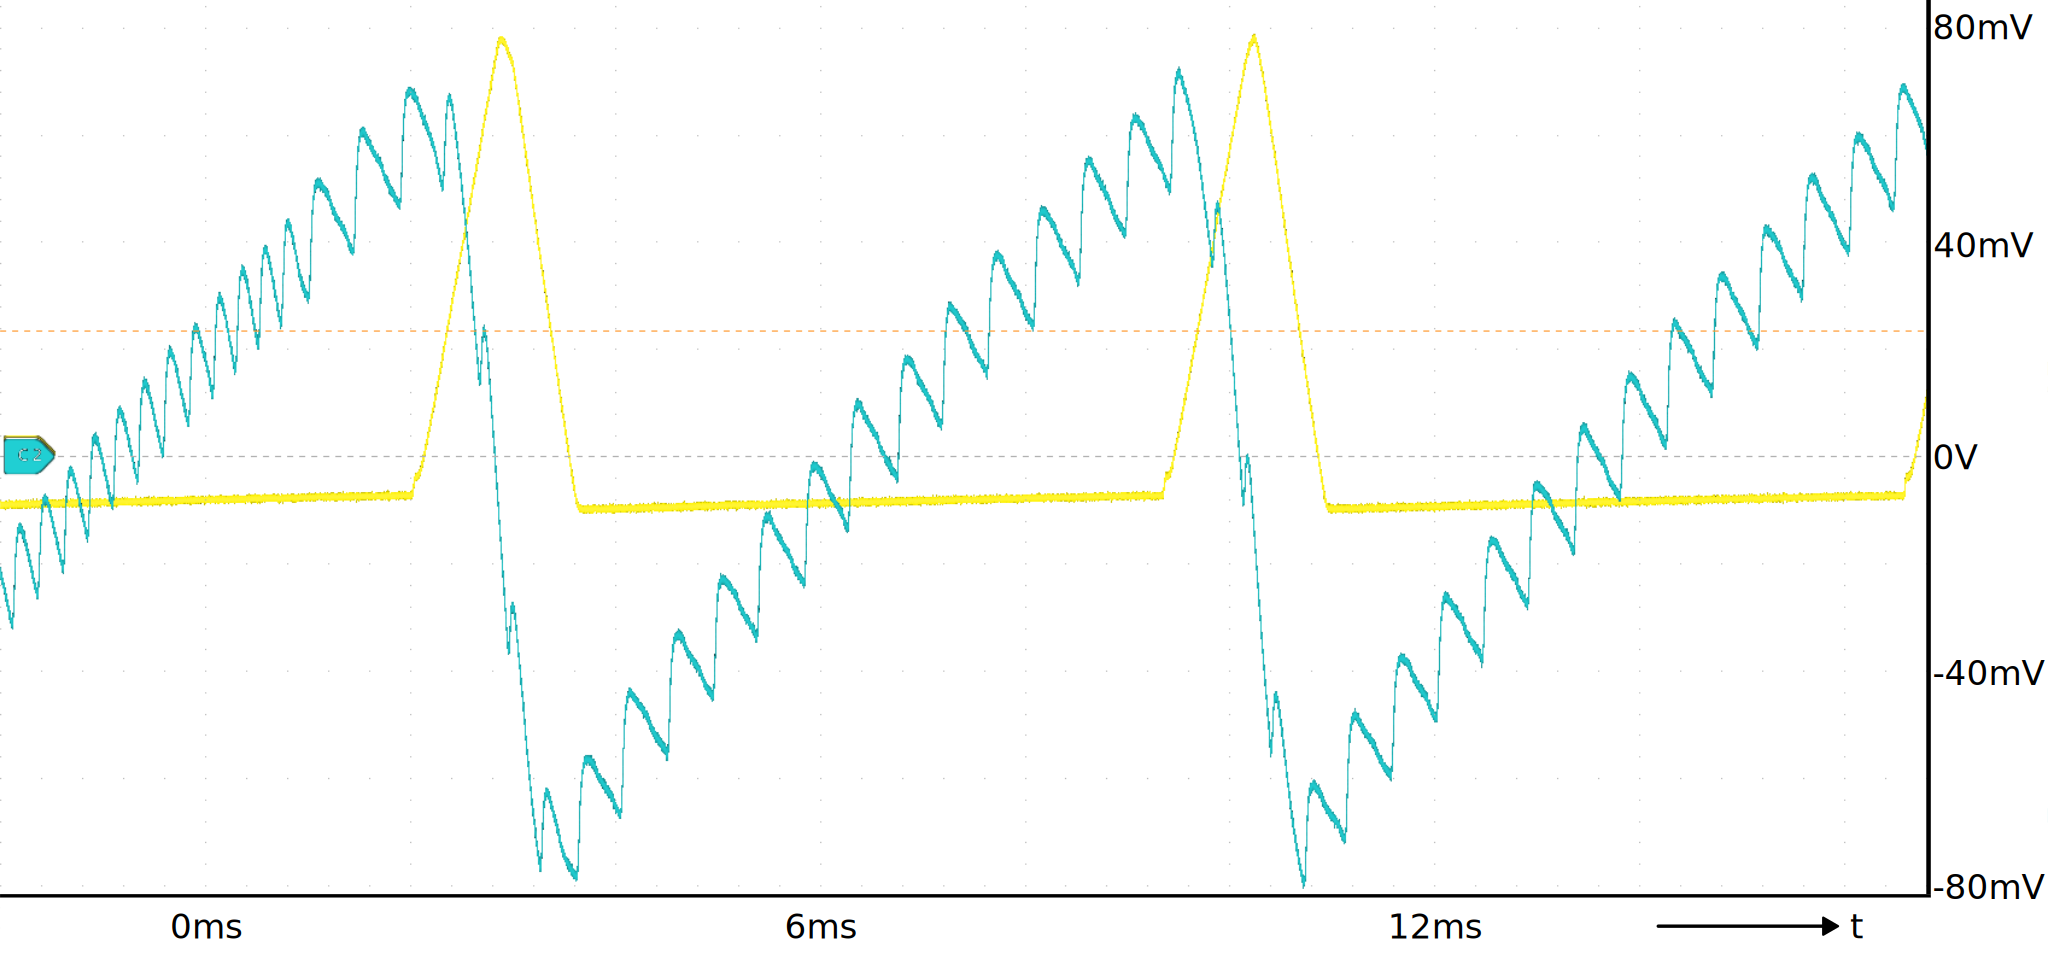
\includegraphics[width=0.8\textwidth]{testUgsUds.png}
    \caption{Het resultaat van de stabiliteitstest. Kanaal 1 (geel) is $U_{gs}$, kanaal 2 (lichtblauw) is $U_{ds}$.}
    \label{fig:resultUgsUds}
\end{figure}


\subsubsection{Discussie}
Er zijn meerdere mogelijke oplossingen voor de instabiliteit.
Eén mogelijke oplossing is een integrator plaatsen tussen de uitgang van de opamp en de gate van de ISFET. Dit zou ervoor zorgen dat de ISFET genoeg tijd heeft om te reageren op de veranderde gate-source spanning, waardoor deze de opamp kan bijhouden.

Een andere mogelijke oplossing is een RC-filter te plaatsen tussen de drain van de ISFET en de niet-inverterende ingang van de opamp. Dit zorgt ervoor dat de opamp trager gaat werken, waardoor de ISFET de opamp bij kan houden.

Er zal een aantal tests gedaan moeten worden om te vinden hoe de ISFET precies reageert op een verandering van de gate-source spanning, en hoe dit verschilt van een reguliere MOSFET. Zo kan een beter model opgesteld worden van de ISFET, waar dan vervolgens een betere uitleesschakeling mee ontworpen kan worden.


\subsection{pH waarde test} 
De volgende test is bedoelt om te testen of het uitgangssignaal verandert op basis van de pH waarde. 

Om te beginnen wordt de uitlees PCB verbonden met de voeding PCB, zodat de uitleesschakeling gevoed wordt. De probe van kanaal 1 van de oscilloscoop wordt verbonden met de ingang van de ADC. De probe van kanaal 2 wordt verbonden met de uitgang van de opamp. Vervolgens worden de ISFET en referentieelektrode in een pH 7 bufferoplossing gestopt. De golfvorm die de oscilloscoop geeft kan nu worden opgeslagen. De meting wordt herhaalt met de ISFET en referentieelektrode in een pH 4 bufferoplossing.

\subsubsection{Resultaten}
De resultaten van deze test zijn te zien in \cref{fig:resultspHMeasure}. Duidelijk is de amplitude van de uitgang van de opamp hoger op pH 7 vergeleken met pH 4.

\begin{figure}[ht]
    \centering
    \begin{subfigure}[b]{0.475\textwidth}
        \centering
        \def\svgwidth{\textwidth}
        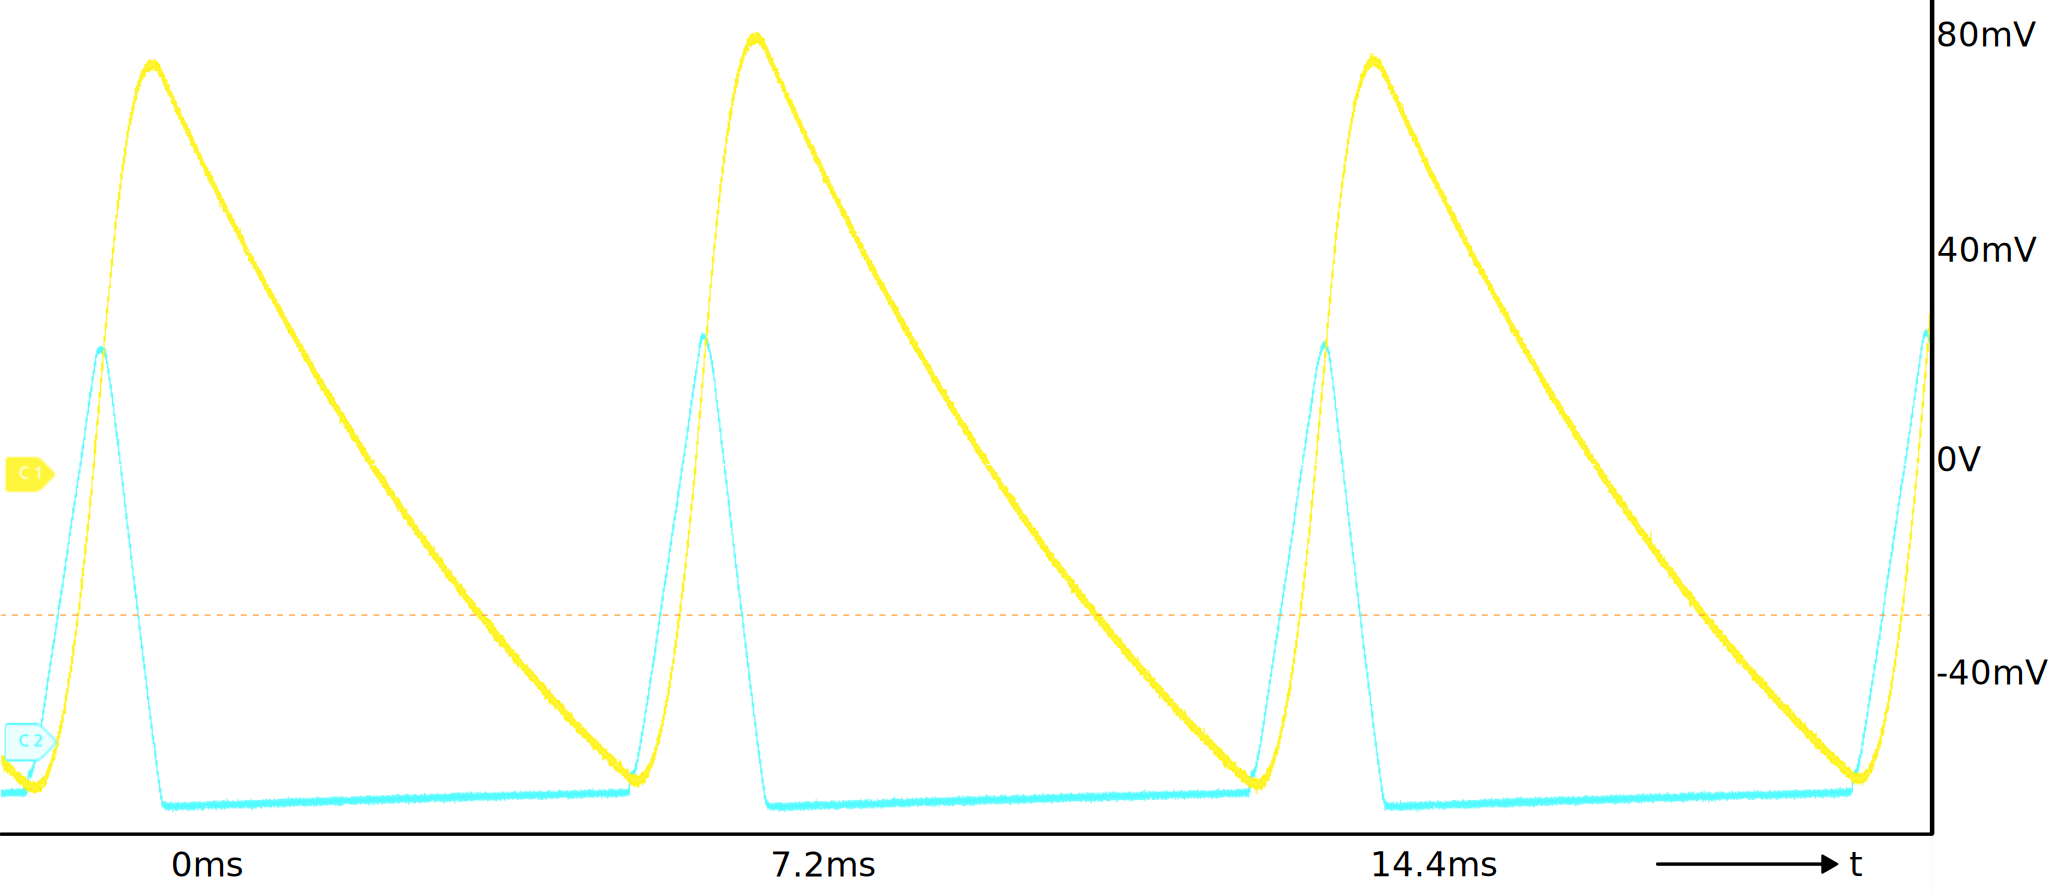
\includegraphics[width=\textwidth]{testpH7.png}
        \caption{De uitgang van de opamp (lichtblauw) en ingang van de ADC (geel) op pH 7.}
        \label{fig:resultpH7}
    \end{subfigure}
    \hfill
    \begin{subfigure}[b]{0.475\textwidth}
        \centering
        \def\svgwidth{\textwidth}
        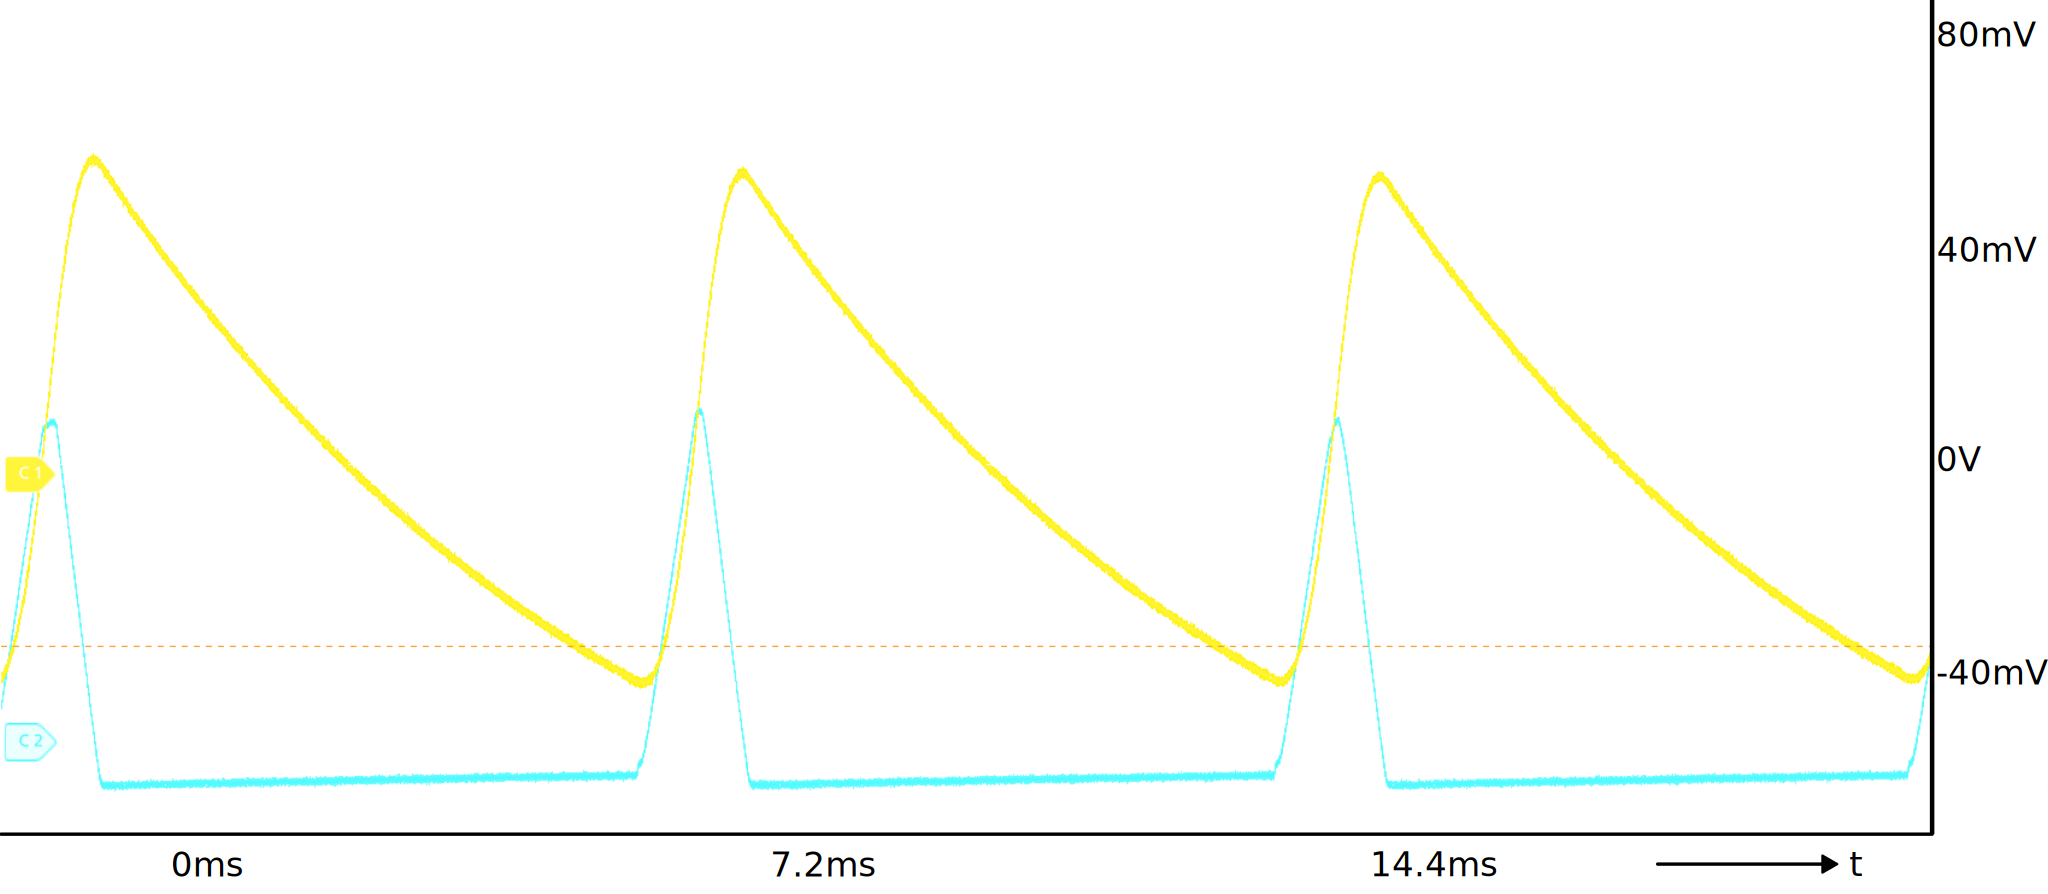
\includegraphics[width=\textwidth]{testpH4.png}
        \caption{De uitgang van de opamp (lichtblauw) en ingang van de ADC (geel) op pH 4.}
        \label{fig:resultpH4}
    \end{subfigure}
    \caption{De uitgang van de meetschakeling op pH 4 en pH 7. Beide metingen hebben dezelfde schaal.}
    \label{fig:resultspHMeasure}
\end{figure}

\subsubsection{Discussie}
Een verandering van pH waarde heeft duidelijk een effect op het uitgangssignaal. Er kan echter nog weinig gezegd worden over de lineariteit van de uitgang op basis van de pH waarde. Hiervoor zou de uitgang eerst stabiel gemaakt moeten worden.


\begin{table}[ht]
    \centering
    \begin{tabular}{l|l|l}
        Apparaat         & Serienummer & Beschrijving \\
        \hline
        MSREF1           & 23/RS03     & Referentie elektrode       \\
        MSFET 3330-2     & 23/205      & ISFET pH sensor            \\
        uitlees PCB      & 1           & ISFET uitlees schakeling   \\
        voeding PCB      & 1           & BMS en energy harvester    \\    
        Keithley DMM6500 & 04458071    & Multimeter spanningsmeting \\
        Keithley DMM6500 & 04458625    & Multimeter stroommeting    \\
        \hline
    \end{tabular}
    \caption{Materialen die zijn gebruikt voor de tests}
    \label{tab:testMaterialen2}
\end{table}


\subsection{Vermogen test}
Deze test is bedoelt om te controleren of het volledige systeem minder dan 10 mW aan vermogen gebruikt. Dit is gedaan door de batterij spanning te meten en de stroom die uit de batterij richting het gehele systeem gaat. Daarvoor zijn 2 Keithley mutlimeters gebruikt. Eén ingesteld op stroom meting modus en geplaatst zodat de batterijstroom door de multimeter gaat. De andere Keithley multimeter is ingesteld om spanning over de batterij klemmen te meten. 

\subsubsection{Resultaten}
De gemeten batterijspanning was 3.82 V, tijdens de loop van de test was deze constant. Het stroomverbruik is tijdens het normaal functioneren van het systeem gemeten tussen 1.3 mA en 2.5 mA. De gemeten stroomwaardes zijn vermenigvuldigd met 3.82V en vervolgens geplot. Deze plot is te zien in \cref{fig:vermogenMeting}. Daarnaast is er een gemiddelde genomen van alle samples om het gemiddelde vermogen te kunnen berekenen. Het gemiddelde vermogen is uitgekomen op 6.81 mW. 

\begin{figure}[ht]
    \centering
    \includegraphics[width=\textwidth]{img/vermogensMeting.pdf}
    \caption{Vermogen meting van systeem}
    \label{fig:vermogenMeting}
\end{figure}

\subsubsection{Discussie}
Uit de metingen is duidelijk te zien dat het hele systeem minder vermogen verbruikt dan de maximale 10 mW die genoemd is in de \cref{sec:systemSpecifications}. 


\subsection{Energy harvesting test}
Voor de energy harvesting test is er een meetopstelling gebruikt waarbij de stroom van en naar de accu gemeten wordt. Vervolgens is het piëzo-element aangesloten op de energy harvesting PCB. Dit element is door middel van een magneet aan de tip van het piëzo-element aan een boormachine kop vastgemaakt. Dit zorgde ervoor dat het piëzo-element bij het draaien van de boormachine vibreerde. Bij deze test is alleen de voeding PCB aanwezig en is de uitlees PCB niet aangesloten.

\subsubsection{Resultaten}
De meting is geëxporteerd en omgezet naar mW, door de gemeten stroom te vermenigvuldigen met de batterijspanning. Dit is zien in \cref{fig:vermogenPlot}.

\begin{figure}[ht]
    \centering
    \includegraphics[width=\textwidth]{vermogen_tijd_plot.pdf}
    \caption{Vermogen meting energy harvesting}
    \label{fig:vermogenPlot}
\end{figure}

\subsubsection{Discussie}
In \cref{fig:vermogenPlot} is te zien dat het energieverbruik van de accu naar 0 mW gaat zodra het piëzo-element genoeg vibreert. Dit toont aan dat de energy harvesting werkt en op lange termijn de levensduur van de sensormodule zal verlengen.


    % \newpage
    % \section{Uitvoering Testplan(nen) en bespreking testresultaten}

    \newpage

    \section{Discussie}
De uitgang van de uitleesschakeling is op dit moment een oscillerend signaal, zoals besproken in \cref{sec:stabilityTestResults}. De ADC geeft echter wel een waarde die proportioneel lijkt te zijn met de pH waarde van de oplossing die gemeten wordt.
De maximumwaardes van de pieken lijken te veranderen op basis van pH. Hiermee is het echter niet mogelijk om de pH nauwkeurig genoeg te bepalen om aan de specificaties uit \cref{tab:systemSpecs} te voldoen.

De energy harvesting piezo produceert op dit moment aanzienlijk minder energie dan op de datasheet gespecificeerd staat. Dit zou kunnen liggen aan de gebruikte testopstelling.

Het gebruikte vermogen dat het systeem gebruikt voldoet aan de \qty{10}{\milli\watt} eis in \cref{tab:systemSpecs}.

\newpage
\section{Conclusie}
De sensormodule kan op dit moment nog niet goed de pH waarde uitlezen. Het vermogensverbruik van de module ligt onder het maximum.


\newpage
\section{Aanbevelingen}
Om het systeem te verbeteren moet uitgezocht worden wat de oscillerende uitgang van de uitleesschakeling veroorzaakt. Dit moet verholpen worden voordat het systeem verder ontwikkeld kan worden. 


% zet misschien nog iets over energiezuiniger maken.
% Noem energie waarde uit illya test.

    \newpage

    \printbibliography[heading=bibintoc]


    \newpage

    % \newpage

    \newpage
    \appendix
    \newpage
    \section{Het bepalen van de path loss fittingscoëfficiënt}
\label{ap:determineFittingsCoef}

\section{Samenvatting}
Om een inschatting te kunnen maken wat het minimale zendvermogen moet zijn voor een bepaalde draadloze applicatie moet er een inschatting worden gemaakt hoeveel signaalverlies er optreed (path loss). In dit meetrapport worden een aantal modellen getoond die hierbij helpen. Een van deze modellen bevat een fittingscoëfficiënt. Door middel van het doen van metingen is er een waarde voor deze fittingscoëfficiënt gevonden.
% intro
% meeting
% conclusie
\section{Abstract}
To estimate the minimum transmission power required for a specific wireless application, it is necessary to assess the anticipated signal loss (path loss). This measurement report presents several models that assist in the estimation of path loss. One of these models includes a fitting coefficient. Through conducted measurements, a value for this fitting coefficient has been determined
\newpage
    \section{Introductie}
% what is pathloss
% When designing wireless electronic systems, end users usually ask for the estimated range of the system. There are two ways that such an estimate can be obtained. The seemingly most simple one of these methods is to just do some measurements. This method is however not able to produce reliable estimates, unless the system has been tested in lots of different environments. The second method on the other hand is centered around equations that predict the signal degradation over distance. This method is also not a perfect prediction thus requiring a fitting coefficient.

Er wordt steeds vaker verlangt dat elektronische ontwerpen draadloos kunnen communiceren. Om er voor te zorgen dat een draadloos systeem een minimaal bereik heeft moet er rekening gehouden worden met signaal verliezen. Een van deze verliezen is path loss. 

% Opdracht en hebben dus model nodig voor path loss in het JMH
% Specificeer frequentie van interesse

% How to calculate path loss 
\subsection{Path loss}
Path loss beschrijft de demping van elektromagnetische golven tussen een zender en een ontvanger. Om deze demping te berekenen, kunnen er verschillende modellen worden gebruikt. In het geval dat de antennes zich in free space bevinden kan \autoref{eq:receivedPowerFreeSpaceIsotropic} gebruikt worden om het ontvangen vermogen te berekenen \cite[13]{bensky2019shortRangeWirelessCommunication}. In \autoref{eq:receivedPowerFreeSpaceIsotropic} zijn \(P_t\) en \(P_r\) de zend en ontvangst vermogens, \(G_t\) en \(G_r\) zijn respectievelijk de zend- en ontvangstversterkingsfactoren van de zend- en ontvangstantennes, \(\lambda\) is de golflengte en d is de afstand tussen de zend- en ontvangstantennes. 
\begin{equation}\label{eq:receivedPowerFreeSpaceIsotropic}
    P_r=\frac{P_tG_tG_r\lambda^2}{\left(4\pi d\right)^2} \,\,\left[\unit{\watt}\right]
\end{equation}
\begin{equation}\label{eq:FreeSpacePathLoss}
    PL_{FS}=20\log\left(\frac{4\pi d}{\lambda\sqrt{G_tG_r}}\right) \,\,\left[\unit{\decibel}\right]
\end{equation}
\begin{equation} \label{eq:isotropicPathLoss}
    PL_{FS}=20\log\left(\frac{4\pi d}{\lambda}\right) \,\,\left[\unit{\decibel}\right]
\end{equation}

Het model dat beschreven wordt met \autoref{eq:FreeSpacePathLoss} gaat er van uit dat de zend- en ontvangende antennes zich free space bevinden. Dit zal echter niet het geval zijn en het model zal dus aangepast moeten worden. Om de reflecties van de grond in het model op te nemen kan het ``two ray model'' als factor aan \autoref{eq:FreeSpacePathLoss} worden toegevoegd \cite{MobileAntenaSystemsHandbookCH2,brini2019system}. 
\begin{equation}\label{eq:twoRayModel}
    PL_{TR}=20\log\left[\frac{1}{1+\Gamma_\bot\exp\left[j\beta \left(\sqrt{\left(h_1+h_2\right)^2+d^2}-\sqrt{\left(h_1-h_2\right)^2+d^2}\right)\right] }\right] \,\,\left[\unit{\decibel}\right]
\end{equation}
\begin{equation}
    -20\log\left[2\sin\left(\frac{2\pi h_th_r}{\lambda d}\right)\right] \,\,\left[\unit{\decibel}\right]
\end{equation}

De voorgaande modellen zijn niet compleet genoeg om de situatie in een bebouwd gebied te voorspellen. Om een beter model te krijgen kan er een fittings factor worden toegevoegd aan \autoref{eq:FreeSpacePathLoss} \cite[24]{brini2019system}. \autoref{eq:fittingFactor} toont deze fittings factor waarin \(l_f\) een fittings coefficient is en \autoref{eq:pathLossModel} toont de resulterende vergelijking voor het berekenen van de verwachte path loss.
\begin{equation} \label{eq:fittingFactor}
    F_f=l_f\log(50d) \,\,\left[\unit{\decibel}\right]
\end{equation}
\begin{equation}\label{eq:pathLossModel}
    PL=20\log\left(\frac{4\pi d}{\lambda}\right)-20\log\left[2\sin\left(\frac{2\pi h_th_r}{\lambda d}\right)\right]+l_f\log\left(50d\right)\,\,\left[\unit{\decibel}\right]
\end{equation}
\begin{equation}
    PL=20\log\left(\frac{4\pi d}{\lambda\sqrt{G_tG_r}}\right)+20\log\left[\frac{1}{1+a_v\exp\left[j\beta \left(\sqrt{\left(h_1+h_2\right)^2+d^2}-\sqrt{\left(h_1-h_2\right)^2+d^2}\right)\right] }\right]+l_f\log(50d) \,\,\left[\unit{\decibel}\right]
\end{equation}

% How to calculate the pathloss fitting coefficient

\subsection{Antenne gain}
    \newpage
    \section{Meetopstelling}

% Description of measurement setup

% Location of measurements

% Table of serial numbers of the used equipement
    \newpage
    \section{Resultaten}
In \autoref{fig:pathLossMesurment:RSS} is te zien wat de gemeten waardes zijn van de testopstelling die is beschreven in \autoref{sec:methods}. Hierbij is de horizontale as de afstand tussen de twee antennes, en is de verticale as het vermogen van de ontvangen signalen.

% place in discussion
%\autoref{fig:pathLossMesurment} toont dat het signaalverlies tussen de ontvangst en zendantennes niet het free space model volgt. 
% Show graph of received power over distance

% Show other results if relevant
\begin{figure}[ht]
    \centering
\begin{tikzpicture}
    \begin{axis}[
        title={},
        xlabel={Afstand (m)},
        ylabel={RSS (dBm)},
        grid=major,
        cycle list name=color list,
        no markers,
        every axis plot/.append style={thick},
        legend pos=outer north east,
        legend style={font=\small}
    ]
    \addlegendimage{empty legend}
    \addplot table [x=Distance,y=-10] {sections/data.dat};
    \addplot table [x=Distance,y=-8] {sections/data.dat};
    \addplot table [x=Distance,y=-6] {sections/data.dat};
    \addplot table [x=Distance,y=-4] {sections/data.dat};
    \addplot table [x=Distance,y=-2] {sections/data.dat};
    \addplot table [x=Distance,y=0] {sections/data.dat};
    \addplot table [x=Distance,y=2] {sections/data.dat};
    \addplot table [x=Distance,y=4] {sections/data.dat};
    \addplot table [x=Distance,y=6] {sections/data.dat};
    \addlegendentry{\hspace{-.6cm}\textbf{TSS}}
    \addlegendentry{-10 dBm}
    \addlegendentry{-8 dBm}
    \addlegendentry{-6 dBm}
    \addlegendentry{-4 dBm}
    \addlegendentry{-2 dBm}
    \addlegendentry{-0 dBm}
    \addlegendentry{-8 dBm}
    \addlegendentry{2 dBm}
    \addlegendentry{4 dBm}
    \addlegendentry{6 dBm}
    \end{axis}
\end{tikzpicture}

%TODO: Add better title?
\caption{RSS (Received Signal Strength) over afstand.}
\label{fig:pathLossMesurment}

\end{figure}

\begin{figure}[ht]
    \centering
\begin{tikzpicture}
    \begin{axis}[
        title={},
        xlabel={Afstand (m)},
        ylabel={PL (dBm)},
        grid=major,
        cycle list name=color list,
        no markers,
        every axis plot/.append style={thick},
        legend pos=outer north east,
        legend style={font=\small}
    ]
    \addlegendimage{empty legend}
    \addplot table [x=Distance,y=-10] {sections/data2.dat};
    \addplot table [x=Distance,y=-8] {sections/data2.dat};
    \addplot table [x=Distance,y=-6] {sections/data2.dat};
    \addplot table [x=Distance,y=-4] {sections/data2.dat};
    \addplot table [x=Distance,y=-2] {sections/data2.dat};
    \addplot table [x=Distance,y=0] {sections/data2.dat};
    \addplot table [x=Distance,y=2] {sections/data2.dat};
    \addplot table [x=Distance,y=4] {sections/data2.dat};
    \addplot table [x=Distance,y=6] {sections/data2.dat};
    \addlegendentry{\hspace{-.6cm}\textbf{TSS}}
    \addlegendentry{-10 dBm}
    \addlegendentry{-8 dBm}
    \addlegendentry{-6 dBm}
    \addlegendentry{-4 dBm}
    \addlegendentry{-2 dBm}
    \addlegendentry{-0 dBm}
    \addlegendentry{-8 dBm}
    \addlegendentry{2 dBm}
    \addlegendentry{4 dBm}
    \addlegendentry{6 dBm}
    \end{axis}
\end{tikzpicture}

%TODO: Add better title?
\caption{Signaalverlies over afstand.}
\label{fig:pathLossMesurment:pathloss}

\end{figure}

\begin{figure}[ht]
    \centering
\begin{tikzpicture}
    \begin{axis}[
        title={},
        xlabel={Afstand (m)},
        ylabel={PL (dBm)},
        grid=major,
        cycle list name=color list,
        no markers,
        every axis plot/.append style={thick},
        legend pos=outer north east,
        legend style={font=\small}
    ]
    \addlegendimage{empty legend}
    \addplot table [x=Distance,y=-10] {sections/data3.dat};
    % \addlegendentry{\hspace{-.6cm}\textbf{TSS}}
    % \addlegendentry{PL}
    \end{axis}
\end{tikzpicture}

%TODO: Add better title?
\caption{Gemiddeld signaalverlies over afstand.}
\label{fig:pathLossMesurment:avaragePathloss}

\end{figure}

\begin{figure}[ht]
    \centering
\begin{tikzpicture}
    \begin{axis}[
        title={},
        xlabel={Afstand (m)},
        ylabel={PL (dBm)},
        grid=major,
        cycle list name=color list,
        no markers,
        every axis plot/.append style={thick},
        legend pos=outer north east,
        legend style={font=\small}
    ]
    \addlegendimage{empty legend}
    \addplot table [x=Distance,y=5] {sections/data4.dat};
    % \addlegendentry{\hspace{-.6cm}\textbf{TSS}}
    % \addlegendentry{PL}
    \end{axis}
\end{tikzpicture}

%TODO: Add better title?
\caption{De mediaan van het signaalverlies over afstand.}
\label{fig:pathLossMesurment:medianPathloss}

\end{figure}
    \newpage
    \section{Discussie}

% Discus the results. 
% Show what the fitting coefficient is after calculation.
    \newpage
    \section{Conclusion}

% Make a conclusion. Broader then the discussion.

% \fbox{
%     \centering
%     \includegraphics[page=1,scale=0.7]{appendix/pathloss.pdf}
% }

% \fbox{
%     \centering
%     \includegraphics[page=2,scale=0.7]{appendix/pathloss.pdf}
% }

% \fbox{
%     \centering
%     \includegraphics[page=3,scale=0.7]{appendix/pathloss.pdf}
% }

% \fbox{
%     \centering
%     \includegraphics[page=4,scale=0.7]{appendix/pathloss.pdf}
% }

% \fbox{
%     \centering
%     \includegraphics[page=5,scale=0.7]{appendix/pathloss.pdf}
% }

% \fbox{
%     \centering
%     \includegraphics[page=6,scale=0.7]{appendix/pathloss.pdf}
% }

% \fbox{
%     \centering
%     \includegraphics[page=7,scale=0.7]{appendix/pathloss.pdf}
% }

% \fbox{
%     \centering
%     \includegraphics[page=8,scale=0.7]{appendix/pathloss.pdf}
% }

% \fbox{
%     \centering
%     \includegraphics[page=9,scale=0.7]{appendix/pathloss.pdf}
% }

% \fbox{
%     \centering
%     \includegraphics[page=10,scale=0.7]{appendix/pathloss.pdf}
% }

% \fbox{
%     \centering
%     \includegraphics[page=11,scale=0.7]{appendix/pathloss.pdf}
% }

% \fbox{
%     \centering
%     \includegraphics[page=12,scale=0.7]{appendix/pathloss.pdf}
% }

% \fbox{
%     \centering
%     \includegraphics[page=13,scale=0.7]{appendix/pathloss.pdf}
% }

% \fbox{
%     \centering
%     \includegraphics[page=14,scale=0.7]{appendix/pathloss.pdf}
% }

\end{document}

%TODO: zoek op "todo"